\documentclass[11pt]{article}
%\documentclass[11pt,dvipdfm]{article}
\usepackage{deauthor,times,graphicx}

% OTHER PACKAGES GO HERE
% List all packages used in your article, eliminating duplicates
% Do not include packages not actually used in your paper
% DO NOT COMMENT OUT PACKAGES, REMOVE THEM
% Ensure that your paper does not include the packages below
% geometry, subfigure, enumitem

% COMMANDS GO HERE
%please list all commands used in your paper, eliminating duplicates

% Your paper submission must be in a folder named with the
% contact author name.

\graphicspath{{submissions/Bolong2023/figs/submissions/Bolong2023/figs/}}
\usepackage{hyperref}
\usepackage{subfig}
\usepackage{url}
\usepackage{multirow}

\usepackage{booktabs}
\usepackage{float}
\usepackage{algorithmicx}
\usepackage{amsmath}
\usepackage{amssymb}
\usepackage{enumitem}
\usepackage{xcolor}
\usepackage{color}
\usepackage{soul}
\usepackage{graphicx}
%\usepackage{amsmath,amsfonts,amsthm}
\usepackage{balance}
\usepackage{threeparttable}
\usepackage{caption}
\usepackage{array}
\usepackage{makecell}
\usepackage{hhline}
\usepackage{array}
\usepackage{enumitem}
\usepackage{threeparttable}

\newcommand{\ie}{\emph{i.e.,}\xspace}
\newcommand{\aka}{\emph{a.k.a.}\xspace}
\newcommand{\wrt}{\emph{w.r.t.}\xspace}
\newcommand{\eg}{\emph{e.g.,}\xspace}
\newcommand{\DD}{\mathrm{\mathcal{D}}}
\def\ie{\emph{i.e.,}\xspace}
\def\cred{\textcolor{red}}
\begin{document}

\title{Approximate Nearest Neighbor Search in High Dimensional Vector Databases: Current Research and Future Directions}

\author{Yao Tian\textsuperscript{$\dagger$}, Ziyang Yue\textsuperscript{$\ddagger$}, Ruiyuan Zhang\textsuperscript{$\dagger$},  Xi Zhao\textsuperscript{$\dagger$}, Bolong Zheng\textsuperscript{$\ddagger$}\thanks{The authors are listed in alphabetical order. Bolong Zheng and Xiaofang Zhou are co-corresponding authors.} , Xiaofang Zhou\textsuperscript{$\dagger$}\textsuperscript{*}
\\
\textsuperscript{$\dagger$}The Hong Kong University of Science and Technology, Hong Kong SAR, China
\\
\textsuperscript{$\ddagger$}Huazhong University of Science and Technology, Wuhan, China\\ 
% \textsuperscript{$\dagger$}\href{zxf@ust.hk}
{\{ytianbc,zry,xzhaoca,zxf\}@cse.ust.hk, \{ziyangyue,bolongzheng\}@hust.edu.cn
% ,
% zry@ust.hk, xzhaoca@cse.ust.hk, zxf@cse.ust.hk
}\\
% \textsuperscript{$\ddagger$}\href{zblchris@gmail.com}{bolongzheng@hust.edu.cn}
}
%\footnote{\textsuperscript{*} The authors are listed in alphabetical order. Boleng Zhang and Xiaofang Zhou are co-corresponding authors}

\maketitle
\renewcommand\thesection{\arabic{section}}
\setcounter{section}{0}
\setcounter{figure}{0}
\setcounter{table}{0}
\begin{abstract}
Approximate nearest neighbor search is an important research topic with a wide range of applications. In this study, we first introduce the problem and review major research results in the past. We then discuss the current work in the database research community, categorizing the work by their key underlying methodologies, such as locality-sensitive hashing, product quantization, and approximate nearest neighbor graphs. Finally, we examine several new directions, with a focus on vector databases to support large language models. 
\end{abstract}

% Body of paper.  The paper should be present as a single file.
% Do not include other files for sections of the paper.
% Papers should not be longer than 12 pages 

% ALL FIGURES MUST BE IN A SUBFOLDER NAMED figs
% See fig-guide for advice about figures
% Your paper's pdf should be less than 500K bytes

% Figures should be include in your paper using 
% the \includegraphics command

% YOUR PAPER GOES HERE

\section{Introduction}
\label{bolong_sec:intro}

\subsection{Dense Vector and Searching}

We are witnessing a notable transition towards vectorized data representations, emerging as the go-to method for encapsulating diverse data forms, from text and images to videos.  This transformation is deeply rooted in the successes of deep neural network-based representation learning. The value of such vector representations is further accentuated by the recent breakthroughs of large language models like ChatGPT and the rapid strides in the multi-modal domain. Specifically, dense vectors representations have gained traction across diverse sectors, including recommendation systems, search engines, and e-commerce, etc.  

To understand the significance of dense vector representations, it is essential to differentiate them from sparse vectors. While sparse vectors contain bits of information distributed sparsely, dense vectors contain the compressed information across every dimension, making them more information rich. Such distinction can be likened to the difference between syntax and semantics in natural language processing. Sparse vectors allow for syntax-based comparisons of sequences, which is efficient in storage. Even if two sentences differ in meaning but share the same syntax, sparse vectors might closely match them. In contrast, dense vectors can be seen as numerical encodings of semantic meaning, which contain their abstract meaning and relationships. Consequently, searches on dense vectors that are derived from text, can be treated as semantic-based searches. This stands in contrast to the traditional syntax-based searches that are typically conducted on sparse vectors.

The adoption of dense vector representations offers clear benefits, including simplicity of data representation and increased computational efficiency. The utility is particularly evident in foundational computational tasks such as search, classification, and clustering, which underpin more complex challenges. Among all operations on dense vectors, the nearest neighbor search, which aims to locate the closest point to a specific reference point, stays in the central position. Unfortunately, it is often infeasible to retrieve the exact nearest neighbors of the query point due to a phenomenon known as “the curse of dimensionality”. As a result, approximate nearest neighbors (ANN) search algorithms have been designed to retrieve the neighbors that are close enough to the reference point. The goal of an ANN search algorithm is to retrieve approximate nearest neighbors of the query point in a low response time,
% maximize \cred{recall??} while retrieving the results as quickly as possible, 
which results in the accuracy-vs-efficiency trade-off  \cite{NEURIPS2019_09853c7f}. 

ANN search is a well-established problem that has garnered significant research attention. The computational complexity is determined by the number of data points ($n$) and the dimensionality ($d$), resulting in a complexity of $O(nd)$. Many existing methods aim to address this challenge by focusing on either reducing the number of data points to examine or decreasing the dimensionality. In terms of reducing the number of data points to examine, two widely employed approaches are space partitioning and proximity graph. Notable methods falling within this category include the $kd$-tree, Approximate Nearest Neighbors Oh Yeah (ANNOY) \cite{annoy}, and the Hierarchical Navigable Small World (HNSW) algorithm \cite{10.1109/TPAMI.2018.2889473}. On the other hand, in the realm of dimensionality reduction, quantization and hashing techniques have gained considerable popularity. Representative methods in this category include Locality-Sensitive Hashing (LSH) \cite{e2LSH}, Spectral Random Sampling (SRS) \cite{SRS}, and Product Quantization (PQ) \cite{DBLP:journals/pami/JegouDS11}.

\subsection{Vector Search Libraries and Vector Database}

The growing need for high-dimensional ANN search in areas such as social media, e-commerce, and digital advertising has shifted the focus from individual algorithms to more integrated libraries. A leading example is Faiss \cite{faiss}, also known as Facebook AI Similarity Search.  Faiss is a C++ library with Python bindings that tailored for the efficient clustering and search of dense vectors. The library encompasses a broad range of similarity metrics and is equipped with widely recognized methods for ANN search, including but not limited to IVFADC \cite{DBLP:journals/pami/JegouDS11}, HNSW \cite{DBLP:journals/pami/MalkovY20}, and LSH \cite{e2LSH}. Notably, Faiss has several GPU-optimized algorithms and seamlessly supports the IVF-PQ series on both CPU and GPU platforms \cite{DBLP:journals/tbd/JohnsonDJ21}. Alongside Faiss, libraries such as ANNOY and Non-Metric Space Library (NMSLIB) provide similar toolkits. ANNOY \cite{annoy} is utilized by Spotify, while NMSLIB \cite{nmslib} has been integrated into Amazon's Elasticsearch Service. Additionally, Alibaba Cloud has introduced a vector analysis framework within their AnalyticDB for PostgreSQL, designed to fetch unstructured data and facilitate association analysis between unstructured and structured data sets.

While libraries like Faiss offer significant capabilities, they might not fully address the complexities of real-world applications. Recognizing this limitation, the concept of vector databases emerges. They are designed much like traditional relational databases but specifically for vector management. They not only offer efficient data indexing, storage, and filtering of vector attributes but also bolster distribution, parallel processing, and facilitate real-time data and index updates. Parallel to the features of a conventional DBMS, they prioritize data safety with backup and collection functionalities. The adaptability is evident in their effortless integration with various data processing tools, analytics platforms, visualization instruments, and AI plugins, enhancing the overall data management workflow. Moreover, these databases are equipped with robust security features and access controls, ensuring the protection of sensitive data, an aspect sometimes overlooked in standalone vector indices. To sum it up, vector databases refine and strengthen the data management landscape with their advanced security and integration capabilities. 

In the vector database domain, Pinecone \cite{pinecone}, Milvus \cite{milvus}, and Weaviate \cite{weaviate} emerge as frontrunners. While all three offer robust solutions for storing, indexing, and searching vast datasets, Pinecone differentiates itself as a closed-source platform. It is exclusively available as a SaaS service, with all user interactions channeled through its API. Conversely, both Milvus and Weaviate are open-source vector databases, benefiting from the collaborative efforts of a varied mix of companies and individual contributors. Some of these participants also extend specialized commercial services and support.

\subsection{Vector Database for LLM}

% With the advancement of large language models like ChatGPT, chatbots have become more sophisticated, serving a wide range of applications. While they are efficient in retrieving information accurately, they also face challenges. These include addressing domain-specific queries, handling hallucination, managing context limitations, reducing query delays, and updating knowledge effectively.

% Vector databases offer potential solutions to the challenges above mentioned. As highlighted, searches on dense vectors, derived from text, are primarily semantic-based. By employing indexing structures for ANNS, vector databases efficiently pinpoint the most semantically relevant information. This allows chatbot models to access a knowledge base where context can be stored for extended durations in a memory-efficient manner. Instead of sourcing context directly from the model, chatbot applications can extract timely and contextually appropriate embeddings from the vector database. This approach not only guarantees more accurate responses, especially for specialized subjects, but also expedites the chatbot's response time, sidestepping the computational demands associated with model retraining or updates.

With the development of large language models such as ChatGPT, chatbots have become more advanced and can now be used for a wide range of applications \cite{DBLP:journals/corr/abs-2303-08774,DBLP:conf/iclr/PatelLRCRC23,DBLP:conf/nips/BrownMRSKDNSSAA20}. While they are effective at accurately retrieving information, they face challenges that can be resolved through vector databases. First, searches on dense vectors derived from text are mainly based on semantics. Vector databases use index structures for ANN search, which enables them to efficiently locate the most semantically relevant information. This allows chatbot models to access a knowledge base where context can be stored for extended periods in a memory-efficient manner. Second, incorporating new data into LLMs without costly retraining is a challenge since current LLMs are static. However, many vector indexes are designed to manage dynamic datasets \cite{DBLP:journals/corr/abs-2105-09613}, which can help extract key information from these datasets when training a new LLM from a trained old one. Finally, data exists in multiple types, and LLMs as a language model do not learn enough about other types of data besides text. Vector databases can help manage these multimodal data in the unified embedding space and feed them to the LLMs. This approach would be a crucial step for LLMs to process various kinds of data sources. Figure \ref{bolong_fig:vdb} shows a framework for enhancing answer quality in LLM-based chatbots. This framework utilizes a vector database as a multi-functional component, serving as a cache, extended memory, and external knowledge base. The vector database not only offers essential indexing and ANN search services but also incorporates comprehensive functionalities expected from a database, including sharding, access control, and query optimization. By leveraging the vector database, the chatbot gains the ability to efficiently retrieve and store relevant information, leading to improved answer quality and enhanced performance.

\begin{figure}
    %\centeringhttps://www.overleaf.com/project/64c1338dcd7ff4dcfaa091bc
    \centering
    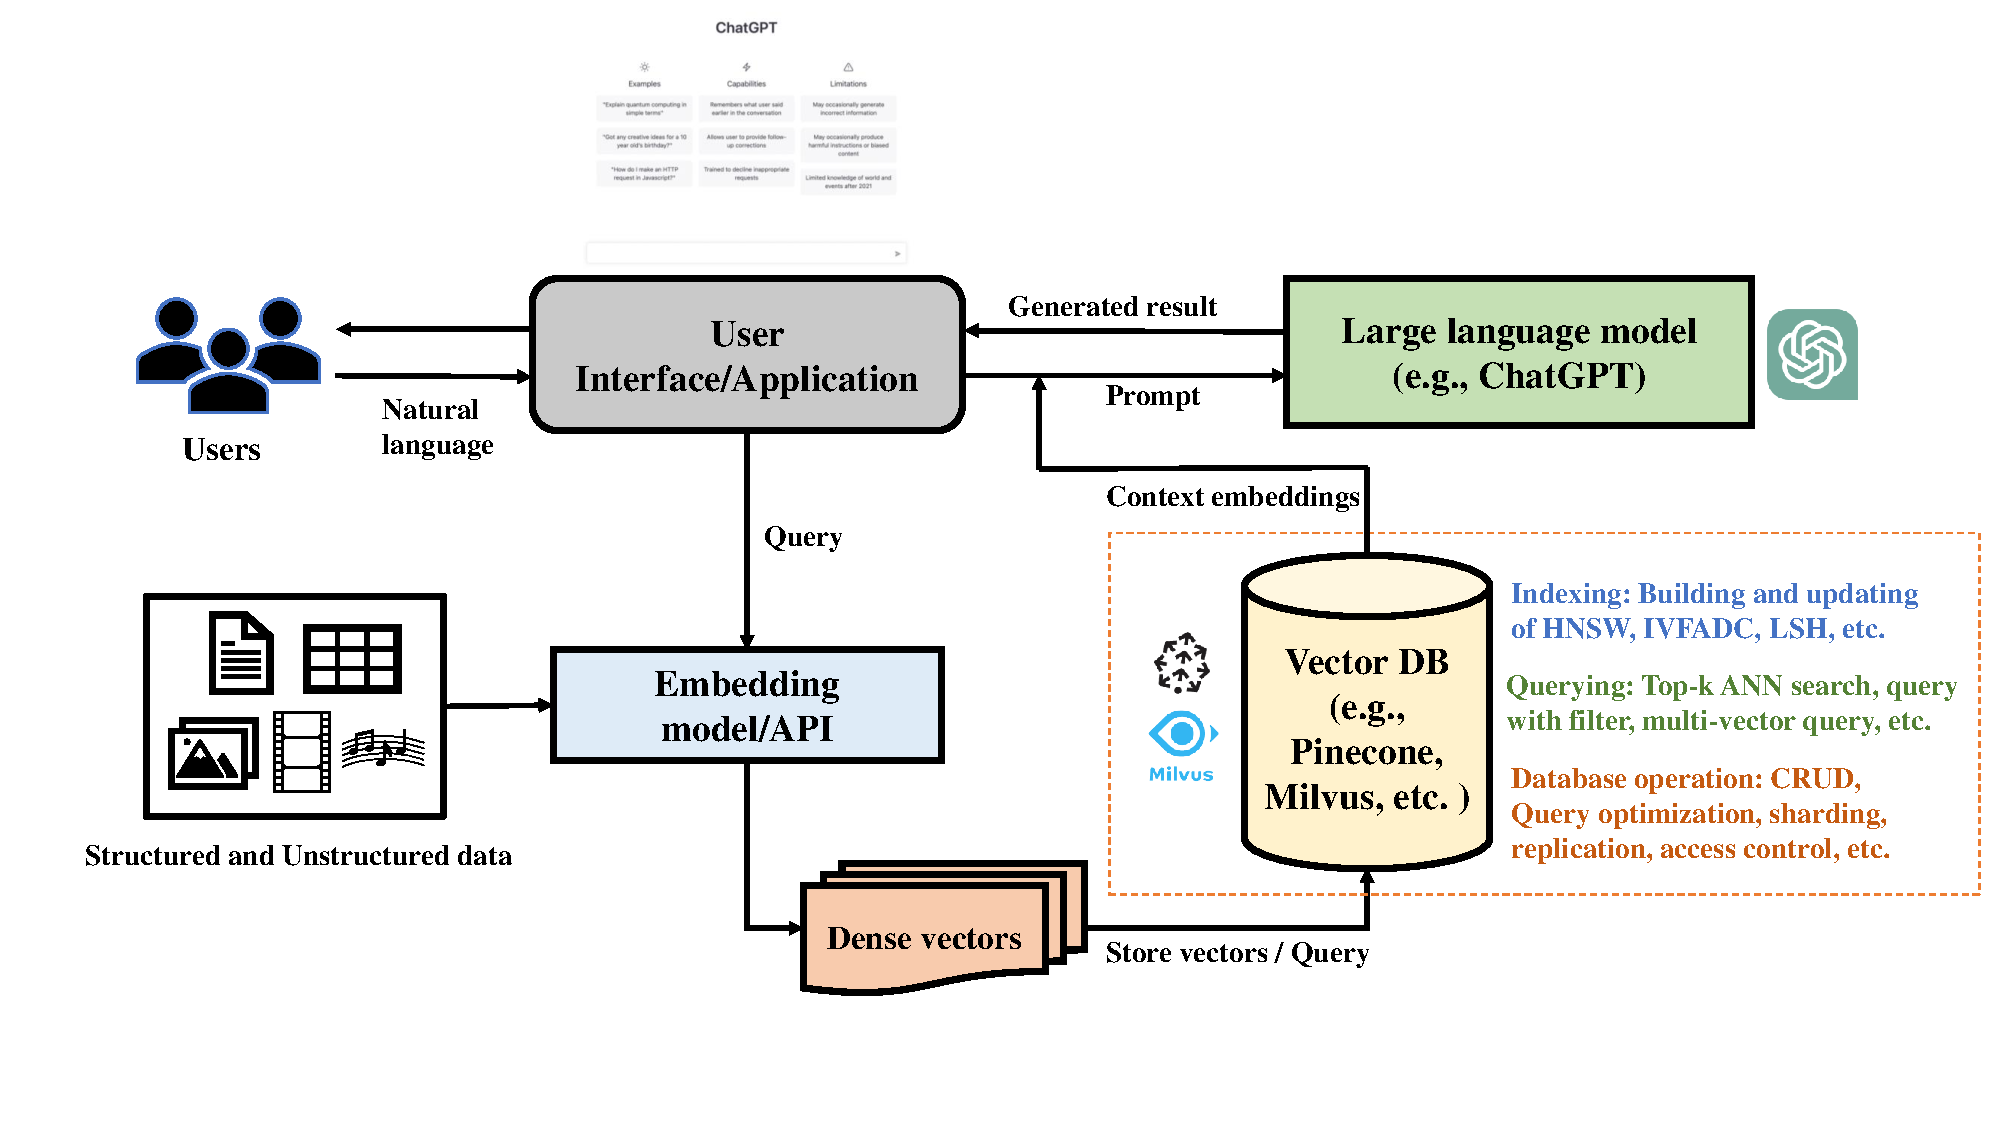
\includegraphics[width=0.9\textwidth]{submissions/Bolong2023/figs/invite_paper_pics_2.pdf}
    \caption{Framework for Enhancing Answer Quality in LLM-based Chatbots using Vector Databases}
    \label{bolong_fig:vdb}
\end{figure}


\subsection{Contribution}

In this study, our objectives are manifold. 1) We delve into the historical trajectory and evolution of the ANN search problem. Based on our research results, we provide a comprehensive overview of the state-of-the-art methods that have been developed. We discuss the foundational principles, key milestones, and the most recent advancements in ANN search. 2) We transition into the challenges that ANN search methods may encounter in the burgeoning era of large language models (LLMs). As the application of ANN search becomes more intertwined with LLMs, a myriad of complexities arise. These challenges span from issues of scalability, where the sheer volume of data can overwhelm traditional methods, to the intricacies of parallel computation, which demands efficient synchronization and communication mechanisms. Furthermore, the need for on-disk indexing introduces another layer of complexity, necessitating efficient data retrieval methods that minimize latency. Additionally, as with any data-centric application, data security remains paramount, prompting rigorous measures to ensure data integrity and confidentiality. 3) We conclude by projecting forward, offering our insights into the potential future research directions in the ANN search landscape. This will encompass emerging trends, potential breakthroughs, and areas that warrant deeper exploration in light of the challenges and opportunities presented by LLMs.

\section{Notation and Preliminaries}
\label{bolong_sec:preliminaries}

We start by clearly defining ANN search. Then, we introduce key index structures used in high-dimensional ANN search. We cover seminal methods such as Locality-Sensitive Hashing (LSH), Product Quantization (PQ), and Hierarchical Navigable Small World (HNSW). The aim is to arm the readers with essential terminologies and foundational concepts, paving the way for the comprehensive discussions that ensue.

\subsection{Problem Definition}
We take $(c,k)$-ANN search in the Euclidean space as an example to illustrate the ANN search problem in high-dimensional spaces. 
Let $\mathcal{D}$ be a set of points in $d$-dimensional Euclidean space $\mathbb{R}^d$ with cardinality $|\mathcal{D}|=n$ and $\|o_1,o_2\|$ denote the Euclidean distance between points $o_1, o_2 \in \mathcal{D}$.

\begin{definition}[$(c,k)$-ANN Search \cite{DBLP:conf/icde/TianZZ22}]\label{bolong_df:ckann}
Given a query point $q$, an approximation ratio $c>1$ and a positive integer $k$, a $(c,k)$-approximate nearest neighbor search returns $k$ points $o_1, \ldots, o_k$ that are sorted in ascending order w.r.t. their distances to $q$. If $o_i^*$ is the $i$-th nearest neighbor of $q$ in $\DD$, it satisfies that $ \|q, o_i\| \leq c\cdot\|q, o_i^*\|$.
\end{definition}

We denote the $(c,k)$-ANN search with $k=1$ as $c$-ANN search. An LSH-based method can ensure a correct $c$-ANN with high probability \cite{DBLP:conf/sigmod/TaoYSK09,DBLP:conf/icde/TianZZ22}. While in the graph-based and quantization-based methods, we usually do not explicitly use $c$ but use \textit{recall} to control the query quality where \textit{recall} measures how many exact $k$NN results is found during the search. 
% \cred{We use recall...? recall is ....?}

\subsection{Seminal Algorithms for High-dimensional ANN Search}

\begin{figure*}[t]
	\centering
	\subfloat[LSH-Based Method]{
		\begin{minipage}[c]{0.32\linewidth}
			\centering
			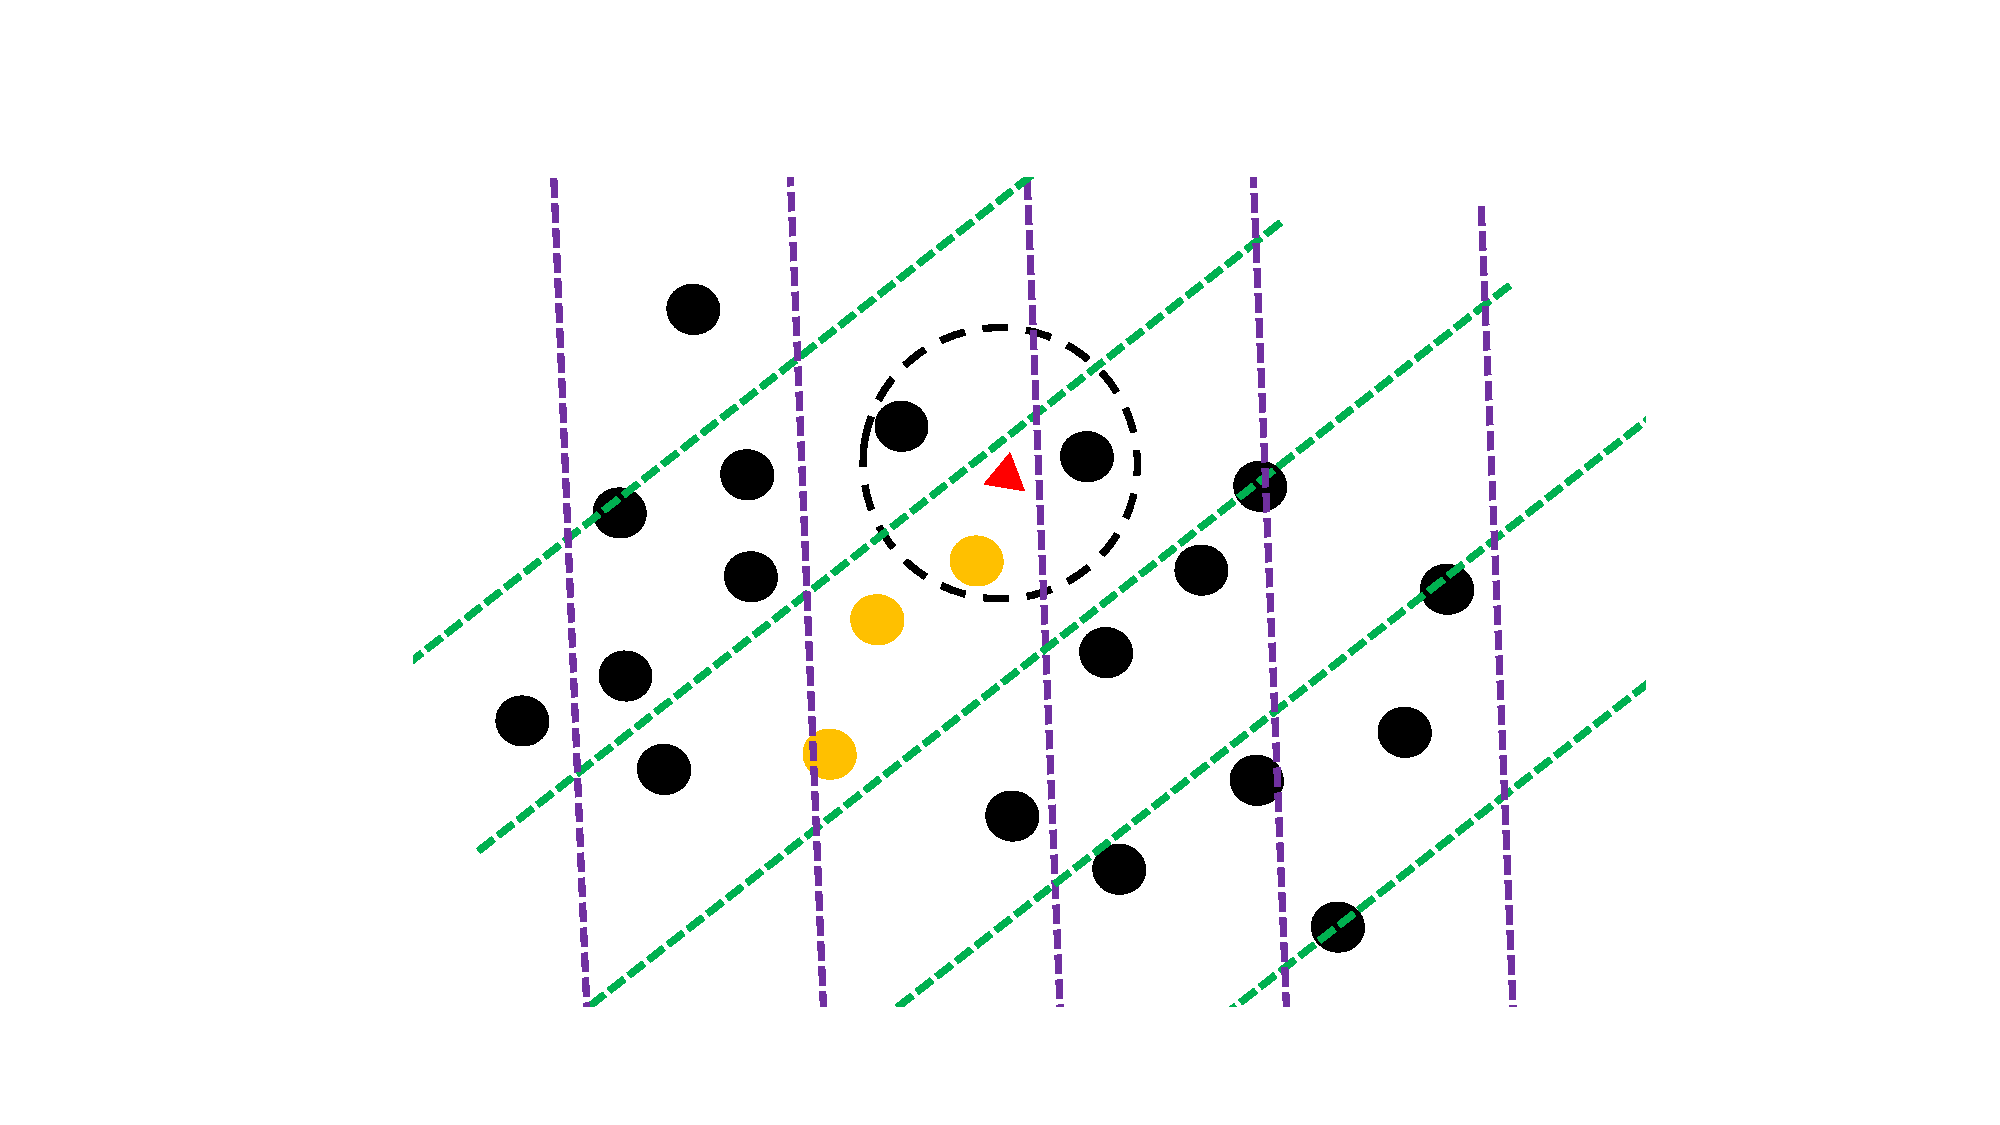
\includegraphics[width=0.95\textwidth]{submissions/Bolong2023/figs/lsh.pdf}
			\vspace{0.5em}
		\end{minipage}
	}
	\subfloat[Quantization-Based Method]{
		\begin{minipage}[c]{0.32\linewidth}
			\centering
			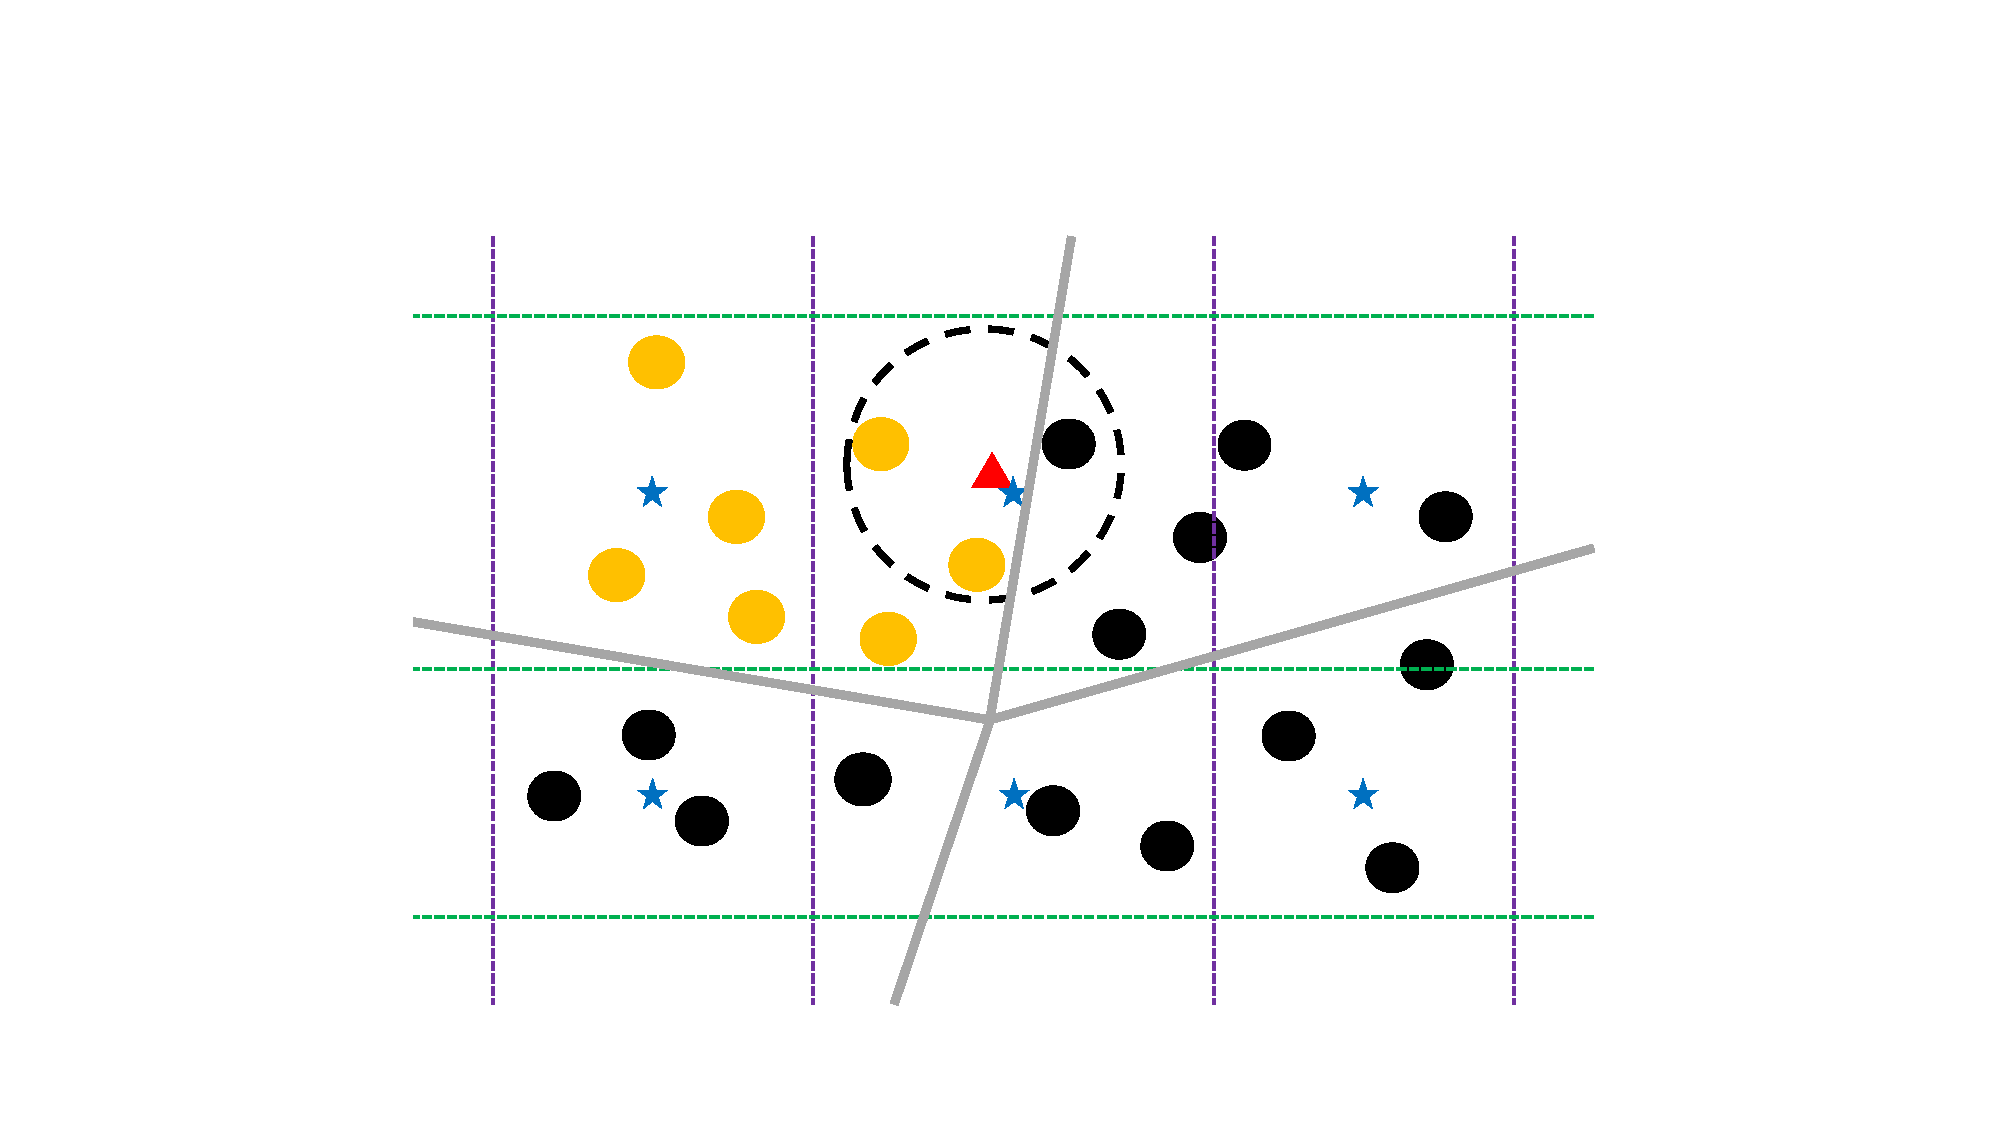
\includegraphics[width=0.95\textwidth]{submissions/Bolong2023/figs/pq.pdf}
			\vspace{0.5em}
		\end{minipage}
	}
	\subfloat[Graph-Based Method]{
		\begin{minipage}[c]{0.32\linewidth}
			\centering
			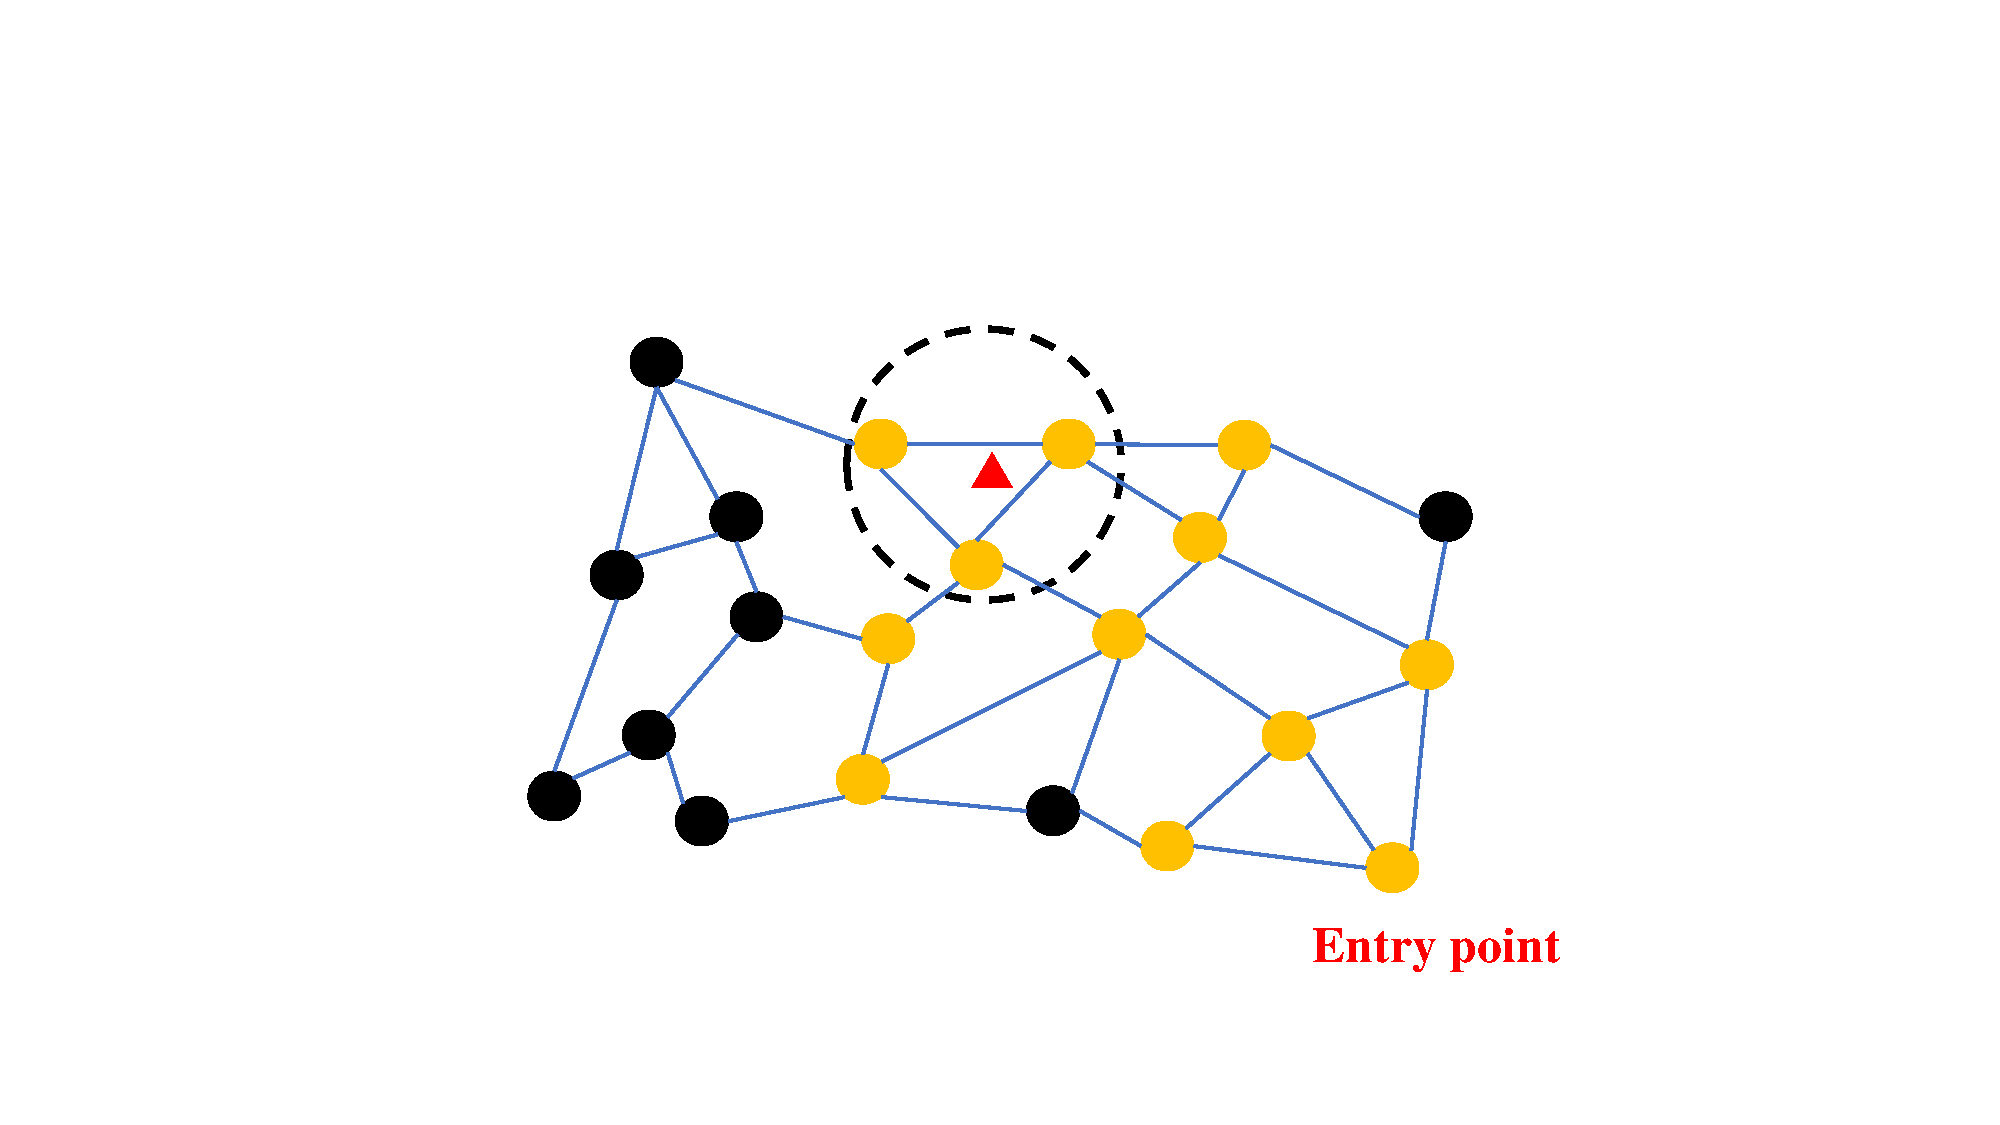
\includegraphics[width=0.95\textwidth]{submissions/Bolong2023/figs/knnG.pdf}
			\vspace{0.5em}
		\end{minipage}
	}
	\vspace{-0.5em}
	\caption{Difference in the LSH-based method, graph-based method and PQ-based method. The red triangle is the query point $q$. The three points in the black dashed circle are the $3$NN of $q$. The orange points denote those that are accessed during the search. 
     % (a) is the LSH-based method. The two groups of parallel lines (purple lines and green lines) are two hash functions and they divide the space into several parallelogram buckets. When conducting the ANN search, we check the points in the bucket where the query point falls. In this example, we find a correct ANN result with cost $3$ but fail to find the exact NN result. (b) is an APG. To simplify the model, we assume the APG is undirected.   Each data point in graph has $2$-$4$ neighbors. The query begins from the bottom right point and approaches to the correct results via greedy search in the APG. All $3$ correct results are found with cost $12$. (c) is LSH-APG. We select the blue point, the closest point to $q$ in the bucket where $q$ falls, as the entry point, and  return all $3$ correct results with a much lower cost $5$.
 } 
%vspace{-0.2em}
	\label{bolong_fig:compare}
\end{figure*}

% \begin{figure*}[t]
% 	\centering
% 	\subfigure[Search in the LSH-Based Method]{
% 		\begin{minipage}[c]{0.32\linewidth}
% 			\centering
% 			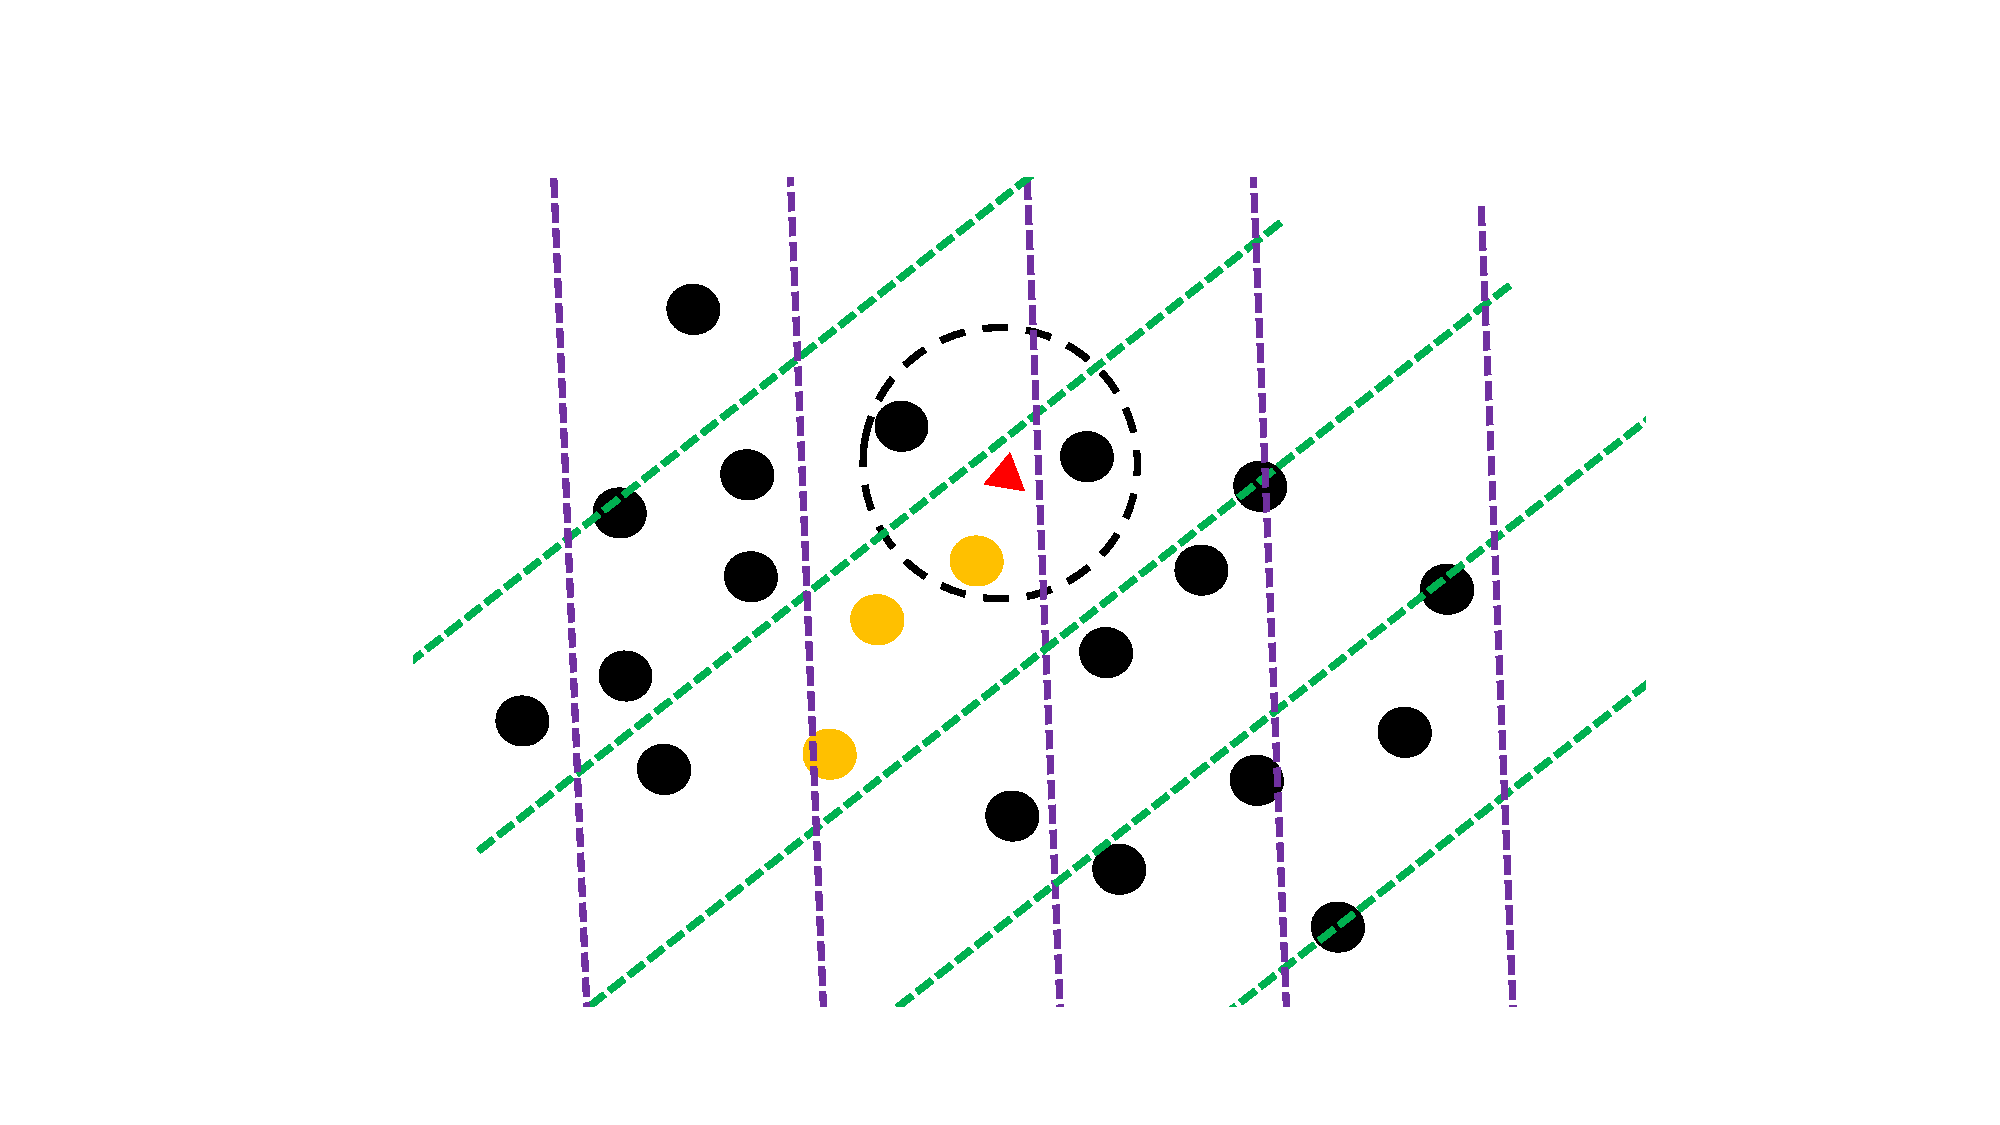
\includegraphics[width=0.95\textwidth]{submissions/Bolong2023/figs/lsh.pdf}
% 			\vspace{0.5em}
% 		\end{minipage}
% 	}
% 	\subfigure[Search in the Graph-Based Method]{
% 		\begin{minipage}[c]{0.32\linewidth}
% 			\centering
% 			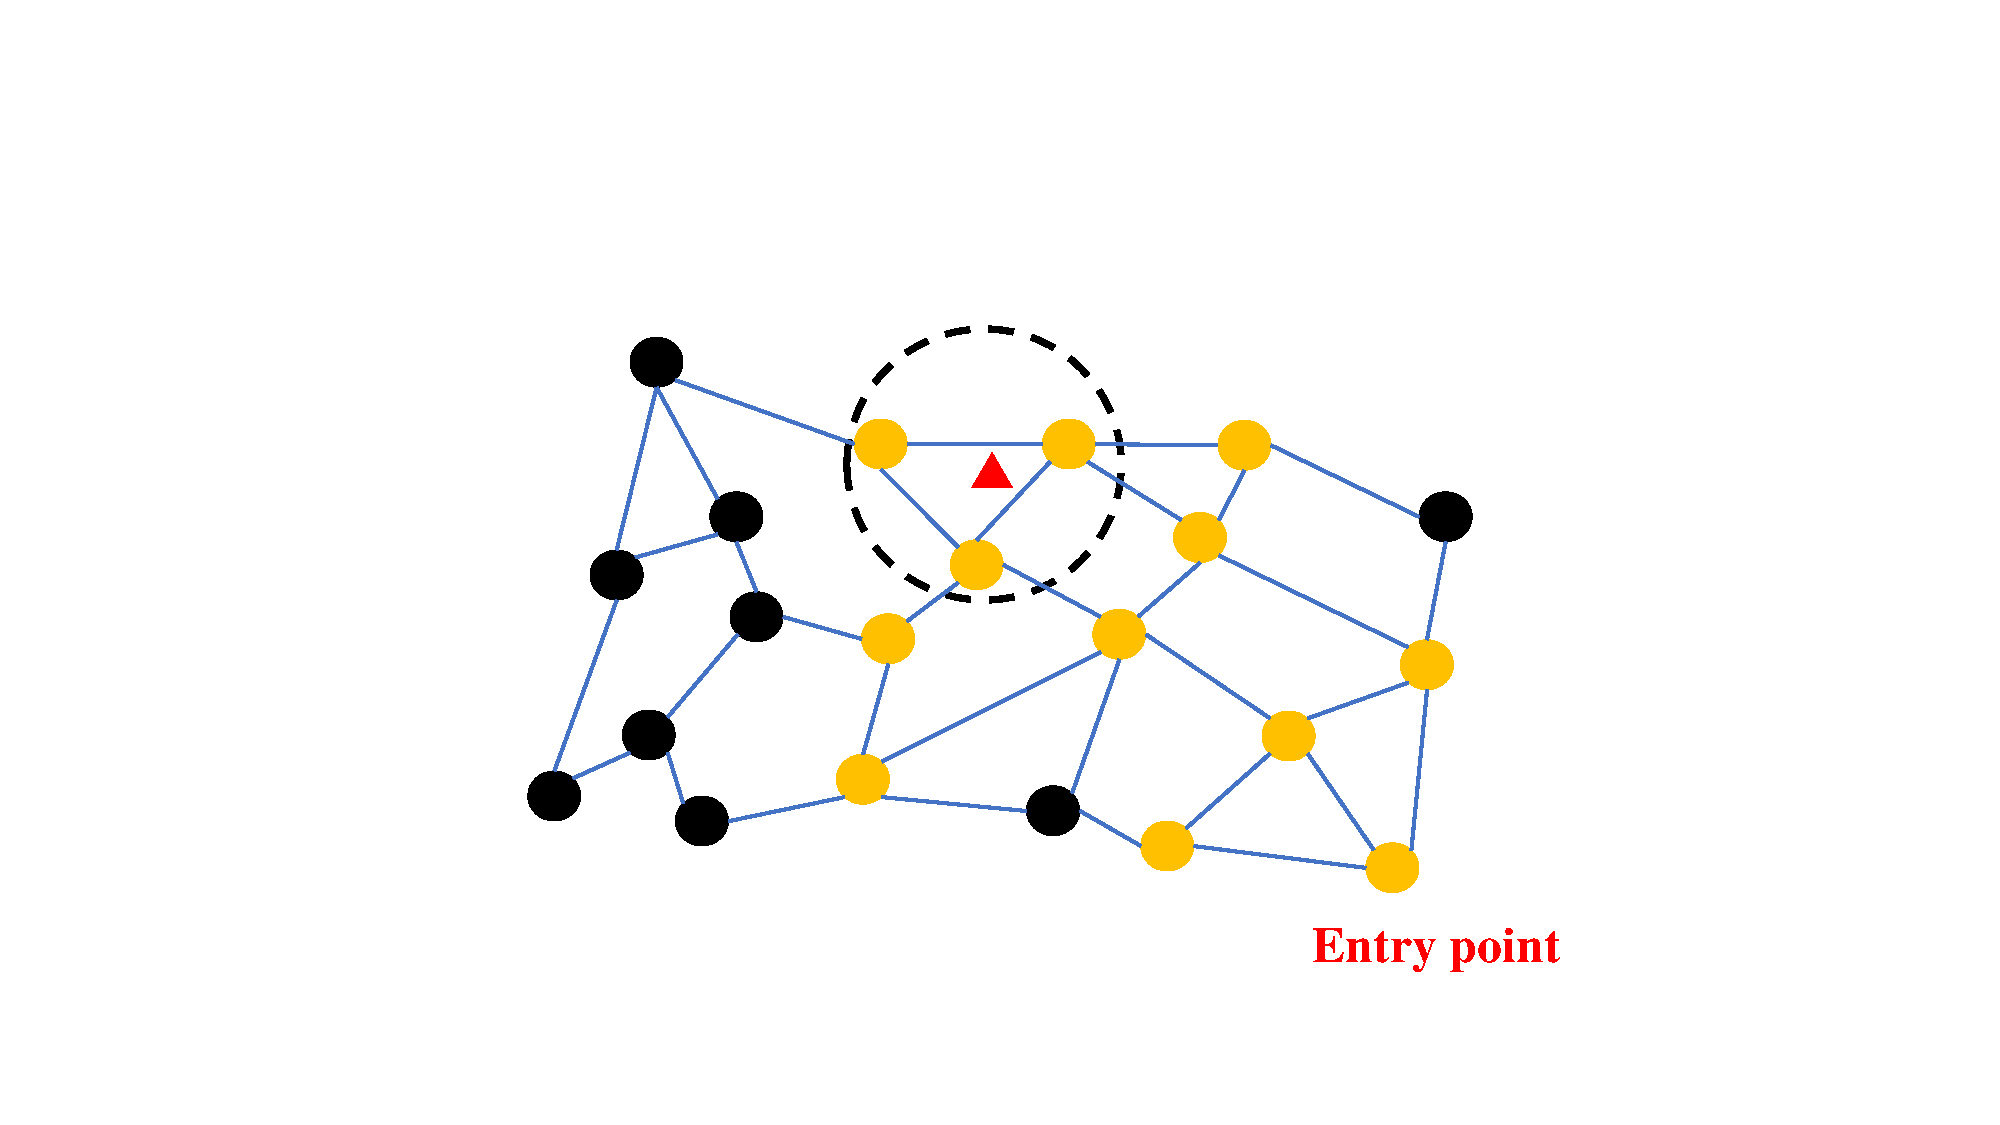
\includegraphics[width=0.95\textwidth]{submissions/Bolong2023/figs/knnG.pdf}
% 			\vspace{0.5em}
% 		\end{minipage}
% 	}
% 	\subfigure[Search in LSH-APG]{
% 		\begin{minipage}[c]{0.32\linewidth}
% 			\centering
% 			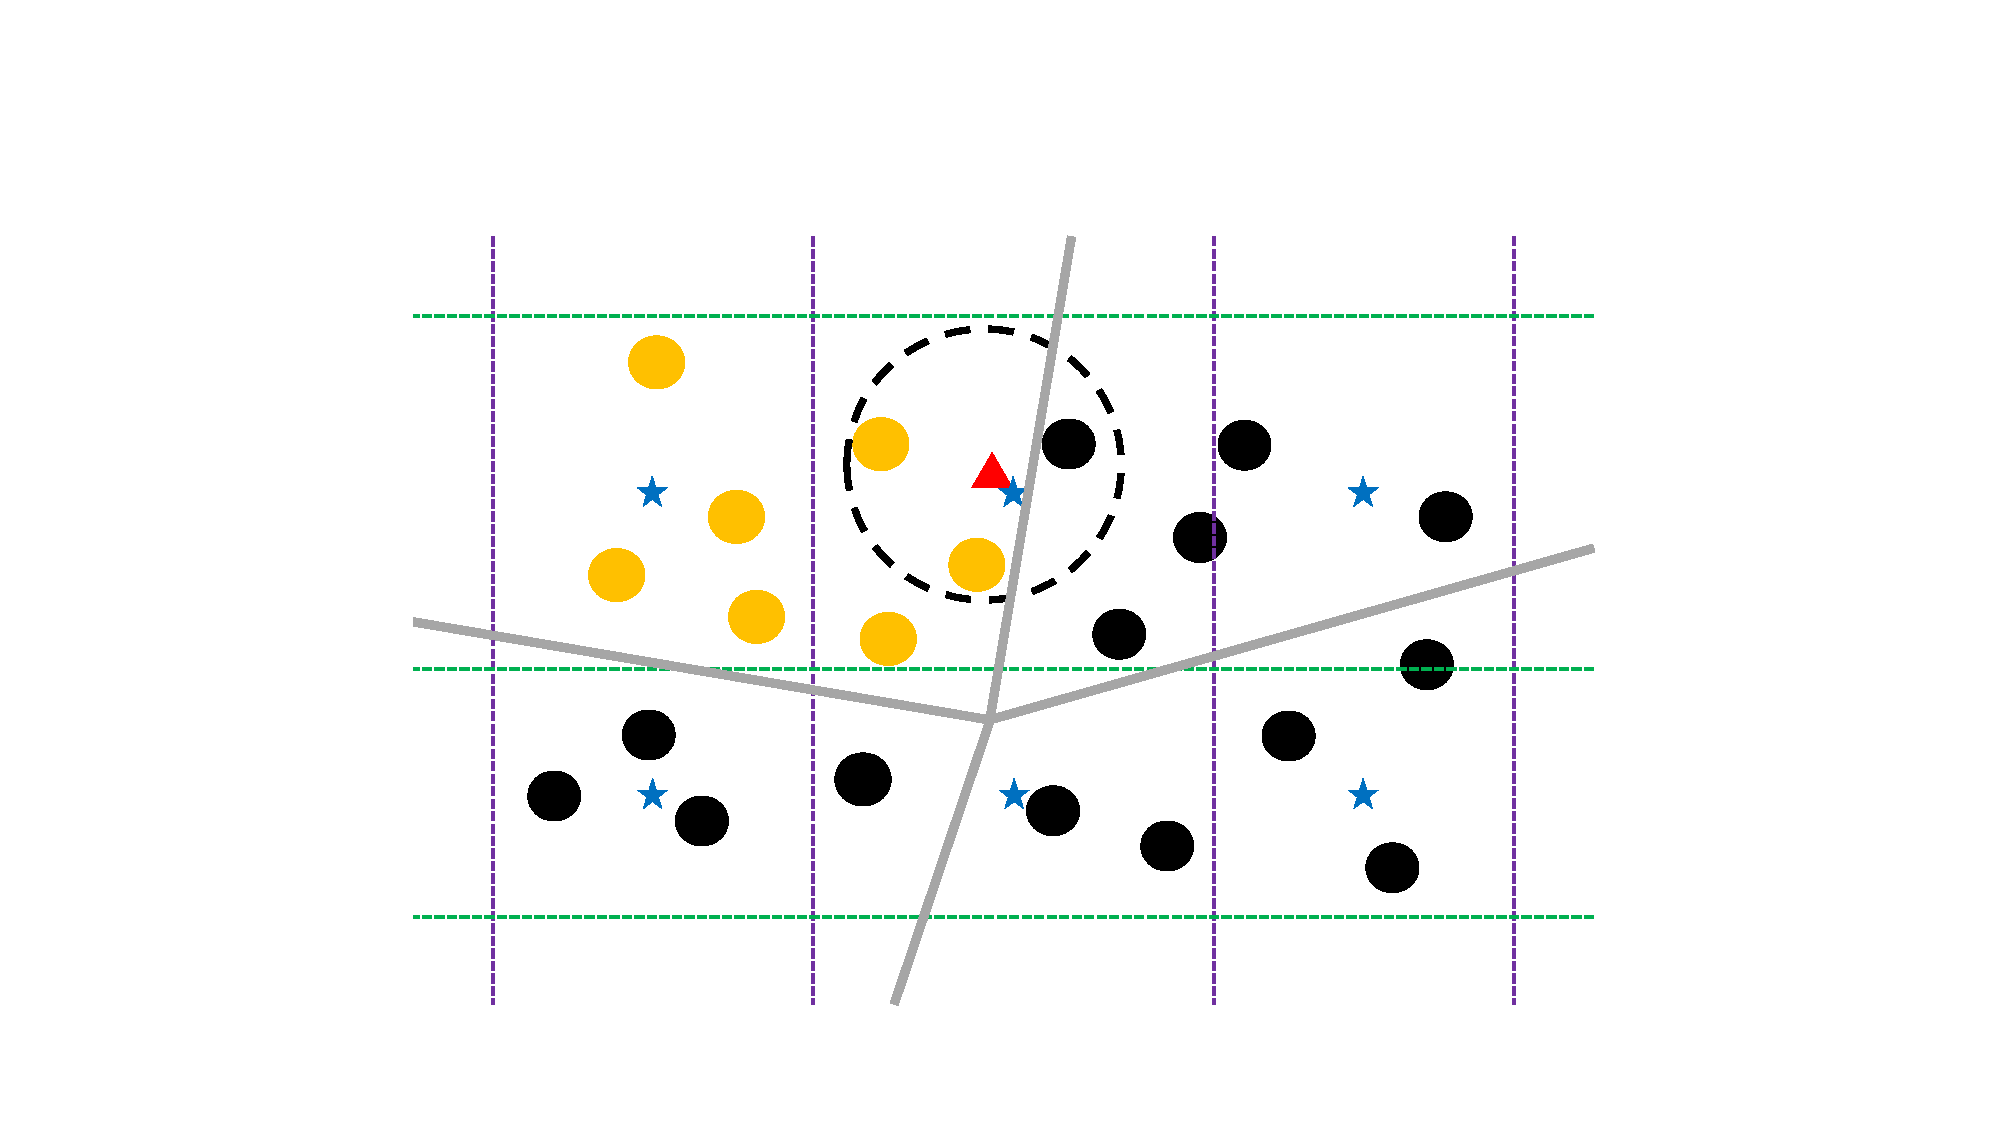
\includegraphics[width=0.95\textwidth]{submissions/Bolong2023/figs/pq.pdf}
% 			\vspace{0.5em}
% 		\end{minipage}
% 	}
% 	\vspace{-0.5em}
% 	\caption{Difference in the LSH-based method, graph-based method and LSH-APG. The red triangle is the query point $q$. The three points in the black dashed circle are the $3$NN of $q$. The orange points denote those that are accessed during the search. 
%      % (a) is the LSH-based method. The two groups of parallel lines (purple lines and green lines) are two hash functions and they divide the space into several parallelogram buckets. When conducting the ANN search, we check the points in the bucket where the query point falls. In this example, we find a correct ANN result with cost $3$ but fail to find the exact NN result. (b) is an APG. To simplify the model, we assume the APG is undirected.   Each data point in graph has $2$-$4$ neighbors. The query begins from the bottom right point and approaches to the correct results via greedy search in the APG. All $3$ correct results are found with cost $12$. (c) is LSH-APG. We select the blue point, the closest point to $q$ in the bucket where $q$ falls, as the entry point, and  return all $3$ correct results with a much lower cost $5$.
%  } 
% %vspace{-0.2em}
% 	\label{bolong_fig:compare}
% \end{figure*}

\subsubsection{Locality-Sensitive Hashing}
Among solutions to the high-dimensional ANN search problem, locality-sensitive hashing (LSH) is known for its sub-linear query time and robust theoretical guarantee of query accuracy. The basic idea behind LSH is to map data points into buckets using a set of hash functions such that nearby points in the original space have a higher probability of being hashed into the same bucket than those far-apart points. 
As shown in Figure \ref{bolong_fig:compare}(a), two groups of parallel lines (purple and green lines) act as two hash functions dividing the space into several parallelogram-shaped buckets. When conducting the ANN search, we check the points in the bucket where the query point falls.
A hash function with such locality-preserving property is called locality-sensitive hashing. LSH was first proposed in \cite{DBLP:conf/stoc/IndykM98,DBLP:conf/vldb/GionisIM99} for the Hamming distance and later extended to several more popular distances, such as the Euclidean distance. E2LSH \cite{e2LSH} is a seminal algorithm for ANN search in the Euclidean space. It adopts the $p$-stable distribution-based function proposed in \cite{DBLP:conf/compgeom/DatarIIM04} as its LSH function. The algorithm concatenates a set of $K (K\ll d)$ independent LSH functions to form a hash table, which is then repeated $L$ times to generate $L$ $K$-dimensional hash tables. Two points in the original space are considered a collision if they are mapped into the same bucket at least once. 
Intuitively, the probability of two different points being hashed into the same bucket increases (or decreases) with $K$ (or $L$). 
% Intuitively, as $K$ increases, the probability of two different points being hashed into the same bucket decreases. On the contrary, the collision probability, which is the probability of two different points being mapped into the same bucket, increases as $L$ increases. 
Theoretical results validate that, with properly chosen values for $K$ and $L$, E2LSH can solve the ANN search problems in sub-linear time with a constant success probability. However, E2LSH needs to prepare a large number of hash tables, which causes large storage costs. Additionally, points close to the query points may be partitioned into buckets different from the one containing the query point, especially when the query is near the bucket boundaries, which jeopardizes the accuracy.

\subsubsection{Product Quantization}
Product Quantization (PQ) \cite{DBLP:journals/pami/JegouDS11} is a widely-used vector quantization technique. It aims to compress high-dimensional vectors into short codes to reduce the space overhead in ANN search. It first divides the $d$ dimensions equally into $M$ groups. Thus each vectors are divided into $M$ sub-vectors and the whole space is divided into $M$ orthogonal $d/M$-dimensional sub-spaces. Then, in each sub-space, sub-vectors are clustered into $K$ groups, and each sub-space centroid is encoded by a single integer code from $1$ to $K$. Finally, each vector can be identified by the concatenation of codes of the nearest sub-space centroid in each sub-space, and the concatenation of the these sub-space centroids is the corresponding quantized vector. In search procedure, the Euclidean distance is replaced by the asymmetric distance as an approximation, which is the Euclidean distance between the query and the quantized vector. The asymmetric distance can be efficiently computed by table lookup and addition of sub-space distances, after the distances between sub-space centroids and sub-vector of query in each sub-space are computed and saved in a distance table. IVFPQ is a variant of PQ, which employs inverted file (IVF) index to index vectors before quantization. Vectors are clustered into different cells, and each IVF list corresponds to one cell and stores the identities of all vectors in it. During ANN search, only vectors located in a few nearest cells are evaluated. Therefore, IVFPQ achieves higher efficiency.
% \cred{To avoid exhaustive evaluation, PQ is often combined with Inverted file index (IVF), thus IVFPQ. Vectors are clustered into different cells and each list in the IVF index stores the PQ codes and identities of vectors from one cell. Only a few nearest cells will be evaluated during search procedure. In this way, Product Quantization achieves low space overhead and high search efficiency.}
As shown in Figure \ref{bolong_fig:compare}(b), the 2D space is divided into two orthogonal 1D sub-spaces with 2 and 3 centroids respectively, thus forming 6 quantizers (the blue stars) in the whole space. Vectors are clustered into 4 cells, and only the nearest one is evaluated during ANN search.

\subsubsection{Proximity Graph}
Graph-based methods have recently come to the forefront as a superior approach for ANN search. They leverage the power of proximity graphs (PG) and have demonstrated superior performance in terms of both accuracy and efficiency \cite{DBLP:journals/pami/MalkovY20,DBLP:journals/pr/MunozGDT19,DBLP:journals/pvldb/WangXY021}.
The fundamental structure of graph-based methods is a proximity graph, represented as $G=(V,E)$. Here, the vertex set $V$ symbolizes all data points in the dataset $\DD$, while the edge set $E$ encompasses all edges between vertices if the corresponding points are sufficiently proximate in the original space. As it is computationally challenging to identify neighbors for each vertex, the construction cost of an exact proximity graph escalates to a minimum of $O(n^2)$ distance computations. This is prohibitively expensive for large-scale datasets. So, even though many well-designed graph structure has been used for nearest neighbor search in multi-dimensional space several decades ago, such as MRNG \cite{DBLP:journals/dam/JaromczykK91}, Delaunay Graph and NN graph, they are hardly adaptive for high-dimensional ANN search problem due to the high indexing cost. Hence, existing graph-based methods concentrate on devising more efficient strategies to construct an approximate proximity graph (APG), such as approximate Delaunay Graph and approximate NN graph, while ensuring robust query performance. 
As shown in Figure \ref{bolong_fig:compare}(c), each data point in graph has $2$-$4$ neighbors. The query begins from the bottom right point and approaches to the correct results via greedy search in the APG.
%\cred{approximate proximity graph (APG) (difference of using APG or PG?)}.


% \section{Nearest Search in High Dimensional Spaces}
% \label{bolong_sec:review}

% In this section, we will give definitions and problem analysis of $k$NN and ANN search in high dimensional space. We will focus on the history of this research, highlighting major work. We need to go beyond the DB area.

% Identifying the nearest neighbor in high-dimensional spaces is a classic and complex task in the database community. With the increasing of the dimensionality of the search space, the "curse of dimensionality" will lead to the phenomenon to the dispersion of data points as the number of dimensions increases, causing them to appear equidistant, thus complicating the tasks of distance-based algorithms. Methods designed to handle lower-dimensional data often do not scale well to high-dimensional settings.

% Initial attempts to address this issue included the use of $kd$-trees, pioneered by Jon Bentley in 1975 \cite{DBLP:kd_tree_bentley}. These data structures divide the space along the dataset's axes, functioning efficiently for low-dimensional datasets. However, as the number of dimensions grows, their performance quickly diminishes, rendering them ineffective for high-dimensional nearest neighbor search.

% Antonin Guttman's R-trees, introduced in 1984, provided an alternative solution for multi-dimensional spatial data. By storing data in minimum bounding rectangles, they facilitated more efficient search operations. However, much like $kd$-trees, they faltered in the face of high-dimensional data, resulting in substantial query processing times.

% In response to these challenges, innovative tree-based structures, such as BallTrees and Cover Trees, were developed. Stephen M. Omohundro proposed BallTrees in 1989, which partition the data space using spheres, whereas Cover Trees, introduced by Alina Beygelzimer, Sham Kakade, and John Langford in 2006, employ a hierarchical organization of the data space. Both structures considerably improved the efficacy of high-dimensional nearest neighbor search.

% Another avenue explored in high-dimensional nearest neighbor search leverages the inherent spatial structure of data. Techniques like Voronoi diagrams and Delaunay triangulation show promise in this regard, offering efficient nearest neighbor queries. However, computing these structures in high-dimensional spaces remains a formidable task.

\section{Current Research Activities}
\label{bolong_sec:architecture}

We proceed to introduce the evolutionary trajectories of the above-mentioned representative categories of indexing structures for ANN search. For each category, we trace its development from inception to its current state, highlighting key milestones and innovations. Additionally, we spotlight the state-of-the-art studies in each category, offering a comprehensive view of the present landscape.


\subsection{Locality-Sensitive Hashing based Methods}
%Among many solutions to the high-dimensional approximate nearest neighbor (ANN) search problem, locality-sensitive hashing (LSH) is known for its sub-linear query time and robust theoretical guarantee of query accuracy. The basic idea behind LSH is to map data points into buckets using a set of hash functions such that nearby points in the original space have a higher probability to be hashed into the same bucket than those far-apart points. A hash function with such locality-preserving property is called locality-sensitive. 
%
%\noindent\textbf{Origins.}
%LSH was first proposed in \cite{DBLP:conf/stoc/IndykM98,DBLP:conf/vldb/GionisIM99} for the Hamming distance and later extended to several more popular distances, such as the Euclidean distance. E2LSH \cite{e2LSH} is a seminal algorithm for ANN searches in the Euclidean space. It adopts the $p$-stable distribution-based function proposed in \cite{DBLP:conf/compgeom/DatarIIM04} as its LSH function. The algorithm concatenates a set of $K (K\ll d)$ independent LSH functions to form a hash table, which is then repeated $L$ times to generate $L$ $K$-dimensional hash tables. Two points in the original $d$-dimensional space are considered a collision if they are mapped into the same bucket at least once. Intuitively, as $K$ increases, the probability of two different points being hashed into the same bucket decreases. On the contrary, the collision probability, which is the probability of two different points being mapped into the same bucket, increases as $L$ increases. Theoretical results validate that, with properly chosen values for $K$ and $L$, E2LSH can solve the ANN problems in sub-linear time with a constant success probability by only checking the points in the bucket where the query point falls. However, to achieve satisfactory accuracy, E2LSH needs to prepare a large number of hash tables, which causes large storage costs. Additionally, points close to the query points may be partitioned into buckets different from  the one containing the query point, especially when the query is near the bucket boundaries because the hash tables are constructed before searching. To remedy these issues, a range of methodologies have been ramified based on different indexing frameworks, alternative search strategies, and elaborate hash functions. 
To remedy the issues with space and hash boundaries in seminal work, a range of methodologies have been ramified based on different indexing frameworks, alternative search strategies, and elaborate hash functions. One such method is Multi-Probe \cite{Multi-probe}, which proposes examining close-by buckets along with the one containing the query point, following an ascending distance score. Rather than utilizing hash tables, LSB-forest \cite{DBLP:conf/sigmod/TaoYSK09} leverages the Z-order curve and B+-trees to index the projected spaces and finds candidates by finding the data point with the greatest Length of the Longest Common Prefix (LLCP). 
LCCS-LSH \cite{DBLP:conf/sigmod/LeiHKT20} introduces the concept of the Longest Circular Co-Substring (LCCS) and a data structure Circular Shift Array (CSA), with which the candidates are identified by the largest LCCS.  These methods carry not only theoretical guarantees of accuracy and efficiency in E2LSH, but also reduce the space cost.
The techniques of Collision Counting and Virtual Rehashing, introduced in C2LSH \cite{DBLP:conf/sigmod/GanFFN12}, offer further space optimization at the cost of query efficiency. Based on the intuition that the incidence of collisions among nearby points tends to exceed that of points distant from each other, C2LSH relaxes the collision criteria from exactly $K$ collisions to any $l$ collisions, where $l < K$ is a given value.  Consequently, C2LSH manages to maintain solely $K$ one-dimensional hash tables, as opposed to the original $L$ $K$-dimensional hash tables. Building upon C2LSH, QALSH \cite{DBLP:journals/pvldb/HuangFZFN15} introduces a query-aware LSH function. By constructing dynamically evolving query-centric buckets, QALSH mitigates the hash boundary issue. R2LSH \cite{DBLP:conf/icde/LuK20} enhances the performance of QALSH by projecting data onto multiple two-dimensional spaces rather than one-dimensional projections. VHP \cite{DBLP:journals/pvldb/LuWWK20} treats QALSH's buckets as hyperplanes, and introduces the concept of a virtual hypersphere to achieve a reduced space complexity. I-LSH \cite{DBLP:conf/icde/LiuWZWQ19} and EI-LSH \cite{DBLP:journals/vldb/LiuW00Q021} introduce an incremental search strategy and a set of adaptive early termination conditions. This strategy enables incremental access to data pointss based on their projected distances and early stops the query process if a good enough result is found. Upon LSH's locality-preserving property, SRS \cite{DBLP:journals/pvldb/SunWQZL14} and PM-LSH \cite{DBLP:journals/pvldb/ZhengZWHLJ20} propose leveraging distances between two points in projected spaces to estimate their corresponding distances in the original space. This enables the determination of ANNs in the original space via lots of exact nearest neighbor searches in projected spaces. These methods rely on a sole multi-dimensional index, yielding gains in space efficiency. However, it's worth noting that the query costs of C2LSH, SRS, and their variants no longer maintain a sub-linear advantage. Concerning hash functions, random linear projections stand out as the prevailing LSH function, while a multitude of studies continue their dedicated efforts to innovate and enhance hash functions and strategies \cite{DBLP:conf/focs/AndoniI06, DBLP:conf/stoc/AndoniR15, DBLP:conf/www/BawaCG05, DBLP:journals/tkde/LiWZWFLW23}.

\subsubsection{DB-LSH: Locality-Sensitive Hashing with Query-based Dynamic Bucketing}
DB-LSH \cite{DBLP:conf/icde/TianZZ22} is a state-of-the-art work that can achieve the lowest query time complexity to date.  It organizes the projected spaces with multi-dimensional indexes instead of fixed-width hash buckets, which significantly reduces space costs.  During the query phase, DB-LSH dynamically constructs query-centric buckets with the required widths and conducts multi-dimensional window queries to  efficiently generate candidates. Different from other query-centric methods, the buckets in DB-LSH are still multi-dimensional cubes like in E2LSH, making it possible to not only generate
high-quality candidates but also to achieve sub-linear query cost. Furthermore, DB-LSH achieves a much smaller bound on query cost compared to existing work, while using an proper and practical bucket size. Rigorous theoretical analysis and extensive experiments show that DB-LSH outperforms the existing LSH methods significantly for both efficiency and accuracy. DB-LSH 2.0 \cite{DB-LSH2} is an extension work of DB-LSH, including DBI-LSH and DBA-LSH. Instead of exponentially enlarging the radius of query window,  DBI-LSH always probes the next best
point in $L$ projected spaces. Such a strategy makes the search terminate at a more proper search radius, and thus can achieve
better accuracy and efficiency. Recognizing the wide variance in the number of candidates required to reach a given accuracy across queries, DBA-LSH is developed on DBI-LSH. This variant incorporates several adaptive early termination conditions by leveraging the intermediate query information, which aggressively reduces the number of points accessed. It has been proven that DBA-LSH can achieve a faster search without breaking the theoretical guarantee.

In summary, LSH-based methodologies offer fast query processing and probabilistic theoretical guarantees of query accuracy.  Moreover, due to their straightforward architecture, LSH-based indexes exhibit quicker construction, streamlined support for updates, and notably smaller index sizes in comparison to alternative approaches for ANN search. Recently, studies adopt the LSH framework to solve other kinds of queries, such as maximum inner product search (MIPS) \cite{DBLP:journals/pvldb/ZhaoZYLXZJ23} and point-to-hyperplane NN search \cite{DBLP:conf/sigmod/HuangLT21} in high-dimensional spaces. These examples demonstrate the superior performance and great flexibility of LSH. Nevertheless, as evidenced by various studies \cite{benchmark}, despite their theoretical assurances, LSH-based methods frequently encounter difficulties in outperforming proximity graph-based and product quantization-based techniques in terms of practical accuracy, a topic that will be delved into in the upcoming sections.

\subsection{Quantization based Methods}
% \subsubsection{Product Quantization}
% Product Quantization (PQ) \cite{DBLP:journals/pami/JegouDS11} is a widely-used vector quantization technique. It aims to compact high-dimensional vectors into short codes to reduce space overhead in Approximate Nearest Neighbor (ANN) Search. PQ first divides the $d$ dimensions equally into $M$ groups. Thus each vectors are divided into $M$ sub-vectors and the whole space is divided into $M$ orthogonal $d/M$-dimensional sub-spaces. Then, in each sub-space, sub-vectors are clustered into $K$ groups, and the sub-space centroids are saved in a codebook, each of which is encoded by a single integer code from $1$ to $K$. Finally, each vector can be identified by the concatenation of codes of the sub-space centroids nearest to the sub-vector in each sub-space, and the concatenation of the these sub-space centroids is the corresponding quantized vector. In search procedure, Euclidean distance is replaced by asymmetric distance as an approximation, which is the Euclidean distance between the query and the quantized vector. Asymmetric distance can be efficiently computed by table lookup and addition of sub-space distances, after the distances between sub-space centroids and sub-vector of query in each sub-space are computed and saved in a distance table. To avoid exhaustive evaluation, PQ is often combined with Inverted file index (IVF), thus IVFPQ. Vectors are clustered into different cells and each list in the IVF index stores the PQ codes and identities of vectors from one cell. Only a few nearest cells will be evaluated during search procedure. In this way, Product Quantization achieves low space overhead and high search efficiency.

Although PQ reduces the space overhead, the process of compression is lossy. The error incurred when vectors are approximated by their quantized vectors, which is called quantization distortion. This results in inadequate search accuracy. Furthermore, due to the coarse-grained structure of IVF index, its effect of pruning deteriorates on large datasets. Therefore, studies on PQ mainly falls in two directions, thus reducing quantization distortion for higher recall \cite{DBLP:conf/cvpr/GeHK013,DBLP:conf/cvpr/KalantidisA14,8404126,Noh_2021_ICCV} and pruning candidates to evaluate for higher efficiency \cite{DBLP:journals/pami/BabenkoL15,DBLP:conf/cvpr/YandexL16,DBLP:conf/sigmod/LiZAH20,DBLP:conf/icde/ZhengYHYLX0J23}.

OPQ \cite{DBLP:conf/cvpr/GeHK013} and LOPQ \cite{DBLP:conf/cvpr/KalantidisA14} attempt to reduce the quantization distortion by introducing rotation matrix. OPQ adopts a global orthogonal matrix to optimize space decomposition. The original space is first transformed by the matrix, and then decomposed in the way PQ does. On the contrary, LOPQ adopts multiple local orthogonal matrices, in order to better fit data with strongly multi-modal distribution. It indexes and partitions vectors with coarse quantizers, and applies a local rotation transformation on residual vectors in each partition. DPG \cite{8404126} uses additional bits to quantize the distance between the vector and corresponding quantizer, because quantization distortion increases when this distance is large. Distance quantizers serve as an error correction term in distance estimation, and improve the search accuracy. Noh et al. \cite{Noh_2021_ICCV} propose a jointly optimization mechanism of coarse and fine quantizers. The coarse quantizers are initialized by K-means, and then optimized with fine quantizers iteratively. In each step, fine quantizers are trained, and each coarse quantizer is updated by the mean error of corresponding vectors.

Some studies are devoted to design more fine-grained index structure to reduce the number of candidates. IMI \cite{DBLP:journals/pami/BabenkoL15} employs the idea of PQ and leverages orthogonal space decomposition to generate inverted indices. Therefore the one-dimensional header in inverted list becomes a multi-dimensional one, and finer partitions are achieved. GNO-IMI \cite{DBLP:conf/cvpr/YandexL16} adopts a non-orthogonal space decomposition method, because orthogonal decomposition cannot fit data with significant correlations between dimensions. It uses two-order clustering to cluster the original vectors and residual vectors respectively, so that each centroid can be represented by the weighted sum of corresponding centroids from two order. Li et al. \cite{DBLP:conf/sigmod/LiZAH20} propose a learned adaptive early termination mechanism in IVFPQ. The gradient boosting decision tree model is build and trained, which takes the query vector and intermediate search results as input features, and decides online whether to early terminate search.
%\textbf{OPQ \cite{DBLP:conf/cvpr/GeHK013} and LOPQ \cite{DBLP:conf/cvpr/KalantidisA14}.} In order to achieve higher recall, OPQ and LOPQ attempt to reduce the quantization distortion by introducing rotation matrix. OPQ adopts a global orthogonal matrix for space decomposition. The original space is first transformed by the orthogonal matrix, and then decomposed into sub-spaces in the same manner as PQ. OPQ takes the quantization distortion as the objective function and seeks for an optimal rotation matrix. Both a non-parametric solution and a parametric solution are proposed. On the contrary, LOPQ adopts multiple local orthogonal matrices, because a single matrix is not enough under strongly multi-modal distribution. LOPQ indexes and partitions the vectors with coarse quantizers, and applies a local rotation transformation on residual vectors (the difference between the vector and its corresponding coarse quantizer) in each partition. In this way, the quantization distortion is further reduced.
%
%\textbf{IMI \cite{DBLP:journals/pami/BabenkoL15} and GNO-IMI \cite{DBLP:conf/cvpr/YandexL16}.} Although IVF index can prune a large portion of vectors far away from the query, its effect deteriorates on large datasets, due to its coarse-grained structure. Therefore, some works turn to design fine-grained index for PQ. IMI employs the idea of PQ and leverages orthogonal space decomposition to generate inverted indices. Therefore the one-dimensional header in inverted list becomes a multi-dimensional one, and finer partitions are achieved. However, when the correlations between dimensions are significant, decomposing the whole space in an orthogonal manner results in many empty cells, so that IMI cannot represent the global data distribution. GNO-IMI adopts a non-orthogonal space decomposition method. It uses two-order clustering to cluster the original vectors and residual vectors respectively, so that each centroid can be represented by the weighted sum of corresponding centroids from two order.
%
%\textbf{Learned Termination \cite{DBLP:conf/sigmod/LiZAH20} and Learned Probing Cardinality \cite{DBLP:conf/icde/ZhengYHYLX0J23}.} A new research trend of PQ is to prune redundant candidate vectors via machine learning or deep learning methods in search procedure. Li et al. proposes a learned adaptive early termination mechanism in IVFPQ. The gradient boosting decision tree model is build and trained, which takes the query vector and intermediate search results as input features, and decides online whether to stop searching. Zheng et al. formally defines the probing cardinality estimation problem (estimate a query-dependent minimized number of cells to probe) and proposed PCE-Net. PCE-Net consists of three encoders and one decoder. The query feature, result quantity feature and IVF index distance feature are encoded by three encoders respectively and then concatenated to feed into the decoder. The decoder outputs the estimated probing cardinality. By replacing fixed search configurations with learned configurations, redundant candidate vectors are reduced and therefore the efficiency of IVFPQ is improved.

% \subsubsection{PCE-IVFPQ}
\subsubsection{Probing Cardinality Estimation IVFPQ}
In IVFPQ and its variants, an input parameter \textit{nprobe} is required. It determines the nearest number of \textit{nprobe} cells to probe, and thus controls the trade-off between accuracy and efficiency. However, it turns out that there is no such a single \textit{nprobe} that is optimal for all queries. Intuitively, if a query locates at the center of a cell, its nearest neighbors may all fall in this cell, so that an $\textit{nprobe}=1$ is enough. On the contrary, if a query locates on the boundary of several cells, we need to set \textit{nprobe} to a large number to include its nearest neighbors distributed in different cells. A fixed \textit{nprobe} will result in that some queries probe either redundant or insufficient cells. Therefore, \textit{nprobe} is an ``impossible-to-set" parameter that should be eliminated.

PCE-IVFPQ (Probing Cardinality Estimation IVFPQ) \cite{DBLP:conf/icde/ZhengYHYLX0J23} formally defines and addresses the probing cardinality estimation problem for the first time. The probing cardinality estimation problem aims to learn a function to estimate a query-dependent minimum probing cardinality (i.e. \textit{nprobe}) for a target recall, given a query vector, a target number of nearest neighbors, and distances between the query and all cell centroids. This problem is a regression problem and can be solved by deep learning techniques. However, using deep learning to estimate probing cardinality faces two main challenges. (1) Due to the sparsity of high-dimensional space, it is difficult to capture the distance distribution between the query vector and database vectors if applying a DNN directly. (2) The data distribution is imbalanced across cells. This results in that the number of vectors to evaluate varies significantly for different queries even with the same \textit{nprobe}, which leads to poor estimation. For the first challenge, specialized modules are designed to process different features. PCE-Net consists of three encoder networks and one decoder network. The query vector, target number of nearest neighbors and distances to all centroids are encoded by three encoders respectively, and then concatenated to feed into the decoder. The decoder outputs the estimated probing cardinality. To mitigate the data distribution imbalance across cells, a hierarchical balanced clustering algorithm is designed, which can generate balanced cells efficiently. Besides, two additional optimization strategies are proposed and further reduce distance computations during cell probing.

In summary, PCE-IVFPQ reduces redundant candidate vectors greatly and achieves the state-of-the-art performance among IVFPQ-based methods w.r.t. search efficiency. The study of probing cardinality estimation is orthogonal to existing studies such as OPQ or IMI, and can be easily adopted by them.

\subsection{Graph based Methods}
% Graph-based methods have recently come to the forefront as a superior approach for Approximate Nearest Neighbor (ANN) search. They leverage the power of proximity graphs (PG) and have demonstrated superior performance in terms of both accuracy and efficiency \cite{DBLP:journals/pami/MalkovY20,DBLP:journals/pr/MunozGDT19,DBLP:journals/pvldb/WangXY021}.
% The fundamental structure of graph-based methods is a proximity graph, represented as $G=(V,E)$. Here, the vertex set $V$ symbolizes all data points in the dataset $\DD$, while the edge set $E$ encompasses all edges between vertices if the corresponding points are sufficiently proximate in the original space. 
% As it is computationally challenging to identify neighbors for each vertex, the construction cost of an exact proximity graph escalates to a minimum of $O(n^2)$ distance computations. This is prohibitively expensive for large-scale datasets. So, even though many well-designed graph structure has been used for NNS in multi-dimensional space several decades ago, such as MRNG \cite{DBLP:journals/dam/JaromczykK91}, Delaunay Graph and NN graph, they are hardly adaptive for high-dimensional ANNS due to the high indexing cost for a long time.

% Existing graph-based methods concentrate on devising more efficient strategies to construct an approximate proximity graph (APG) while ensuring robust query performance. 
Efficiently constructing an Approximate Proximity Graph (APG) is a significant challenge when designing a graph-based index. Various strategies have been proposed to address this challenge. 
NN-Descent is a prevalent technique for constructing approximate Nearest Neighbor (NN) graphs. This method involves building an Approximate Proximity Graph (APG) from a random graph, with the edges for each point updated iteratively through a local search among the query's close neighbors. The construction complexity of NN-Descent is reduced to $\tilde{O}(n^{1.14})$, making it significantly more efficient than brute-force methods. The NN-Descent algorithm is employed in numerous graph-based approaches, such as EFANNA \cite{DBLP:journals/corr/FuC16}, NSG \cite{DBLP:journals/pvldb/FuXWC19} and others \cite{DBLP:journals/corr/abs-1804-03032,DBLP:journals/corr/abs-1908-00814}. Several derivatives of this algorithm have also been developed \cite{DBLP:conf/wims/BraticHKOR18}.
On the other hand, the Hierarchical Navigable Small World (HNSW) algorithm constructs its graph by sequentially inserting points. When inserting a point, denoted as $o$, the number of layers $o$ should be placed in is determined through a random number. A query is then conducted for $o$ in the current index, and $o$'s neighbors are chosen from the obtained results. Additionally, HNSW employs an edge occlusion rule to decrease the out-degree, a procedure proven to be identical to the one used in NSG. This rule enhances the distribution diversity of neighbors and boosts query efficiency. Known for its superior performance in addressing the ANN search problem, HNSW is implemented in several widely-used libraries like NMSLib \cite{nmslib} and Faiss \cite{faiss}, which offer efficient tools for similarity search.

%While APG emerges to be the most promising methods for solving ANN problem, it becomes a challenge to update APGs for dynamic datasets. 
%As the dataset evolves, many points in the proximity graph requires to be inserted and deleted. 
%Inserting a point in the APG is rather easy by using the similar strategy as consecutive insertion strategy. However, it is hard to delete points in the APG since the point is connected to other points and there are many edges required to be dropped. There are two typical policies to address the deletions in an APG. The first policy is to drop graph vertices corresponding to deleted points. The points, including its in-edges and out-edges are all deleted. The biggest problem of this policy is that it will make some vertex connected to it become sparse, \ie the number of edges of these points is small, which will degrade the graph quality.
%The second policy is that when deleting vertex $o$, for any pair of directed edges $(o_{in}\to o)$ and ($o\to o_{out}$) in the graph, we add the edge ($o_{in}\to o_{out}$) in the updated the edge set of $o_{in}$. 
%This policy address the problem in the former policy and ensures the graph quality not to degrade during updating but heavily increases the deletion cost because it is time-consuming to update the edge sets of all $o_{in}$s. So, it is challenging to ensure the graph quality and update efficiency when updating APGs.
While APG has emerged as the most promising method for solving ANN search problems, updating APGs for dynamic datasets can be quite challenging. As the dataset evolves, many points in the proximity graph need to be inserted and deleted. Inserting a point in the APG is relatively easy using the same strategy as the consecutive insertion strategy. However, deleting points in the APG is difficult as the point is connected to other points and many edges need to be dropped. There are two typical policies to address deletions in an APG \cite{DBLP:journals/corr/abs-2105-09613}. The first policy is to drop graph vertices corresponding to deleted points, including their in-edges and out-edges. However, this policy can make some vertices connected to it become sparse, resulting in a degradation of graph quality. The second policy is that when deleting vertex $o$, for any pair of directed edges $(o_{in}\to o)$ and $(o\to o_{out})$ in the graph, we add the edge $(o_{in}\to o_{out})$ in the updated edge set of $o_{in}$. This policy addresses the problem in the former policy and ensures the graph quality does not degrade during updating, but heavily increases the deletion cost because it is time-consuming to update the edge sets of all $o_{in}$s. Therefore, ensuring graph quality and update efficiency when updating APGs is a challenging task.

\subsubsection{{Locality Sensitive Hashing-Approximate Proximity Graph}}
Locality Sensitive Hashing-Approximate Proximity Graph (LSH-APG) \cite{DBLP:journals/pvldb/ZhaoTHZZ23} is an innovative graph-based method that leverages lightweight LSH indexes to construct the APG and expedite ANN search processing. 
LSH indexes, while swiftly constructed, often fall short in terms of query accuracy. On the other hand, graph-based methods excel in query processing performance but are hindered by the high construction cost due to their intricate construction and edge selection strategies. 
LSH-APG aims to mitigate these limitations inherent in both LSH and graph-based methods. It utilizes LSH indexes to quickly retrieve preliminary query results as the starting point for a search in an APG, then employs graph-based techniques to further refine the accuracy of the query result. 
In a departure from HNSW and NSG, which reduce the number of edges based on the edge occlusion rule, LSH-APG introduces an accurate and scalable pruning strategy to filter out neighbors distant from the query point. This approach markedly reduces the number of points accessed during graph search, effectively boosting query efficiency without increasing the construction cost. 
To construct the graph index, LSH-APG employs the consecutive insertion strategy where LSH framework can help find the candidate neighbors. All points are consecutively incorporated into the APG, where each point is treated as a query point and inserted into the graph index based on its nearest neighbors. It addresses the issue of high construction cost with the assistance of the LSH framework.
This strategy not only curtails construction cost by enhancing search efficiency via the LSH framework, but also allows for a formal correctness and complexity analysis of LSH-APG. The theoretical result show that LSH-APG have a nearly $O(n)$ query cost. 

%Moreover, LSH-APG designs a "mark-and-delete" policy to alleviate for index update, which pursues for a good balance between the graph quality and updating efficiency. To delete a point $o$ in the graph indexes, LSH-APG first marks the points $o$ and all of its out-edges. We usually only store the out-edges but not in-edges in APGs. Finding in-edges is also an uneasy task to be considered in the above two policies. 
%LSH-APG adopts a approximate query algorithm to find the in-edges. The query cost is bounded by a given threshold $C_{Dm}$ to control the deletion efficiency. Then, for an in-edge of $o$ not found in the range search, we leave it to the deletion procedure in the following queries. If it is found during an ANN query later, we discard it and decrease the in-degree of $o$ by one. Once the in-degree of $o$ becomes $0$, we discard all the out-edges of $o$ and $o$ itself. Finally, to avoid some in-edges not being found for a long time and thus wasting the space, we also traverse the graph and discard all the edges to be deleted when their amount reaches 10$\%$ of the total number of edges in LSH-APG. To ensure the graph quality, LSH-APG controls the out-degree of each vertex to be within an interval $[T,2T]$. So, when we mark an edge $(u,o)$ as deletion, we will check whether $u$'s out-degree decreases to be less than $T$. If so, we will increase the number of $u$'s neighbors to $T'$ by finding points in neighbors of $u$'s neighbors. By this manner, LSH-APG reduces the bad influence of the deletion on the graph quality with an acceptable cost.
Furthermore, LSH-APG has designed a ``mark-and-delete" policy to alleviate index update issues, which aims to strike a balance between graph quality and updating efficiency. To delete a point $o$ in the graph indexes, LSH-APG first marks $o$ and all its out-edges. Typically, only out-edges are stored in APGs, and finding in-edges is a challenging task that is not considered in the previous two policies. To address this, LSH-APG uses an approximate query algorithm to find the in-edges, with the query cost bounded by a given threshold $C_{Dm}$ to control deletion efficiency. If an in-edge of $o$ is not found in the search, it is left for deletion in subsequent searches. If it is found during an ANN search later, it is discarded, and the in-degree of $o$ is decreased by one. Once the in-degree of $o$ becomes zero, all its out-edges and $o$ itself are discarded. To prevent in-edges from occupying space for an extended period, LSH-APG also traverses the graph and discards all edges to be deleted when their number reaches 10$\%$ of the total number of edges in LSH-APG. To ensure graph quality, LSH-APG controls the out-degree of each vertex to be within the interval $[T,2T]$. When an edge $(u,o)$ is marked for deletion, LSH-APG checks whether $u$'s out-degree decreases to less than $T$. If so, the number of $u$'s neighbors is increased to $2T$ by finding points in the neighbors of $u$'s neighbors. This approach reduces the negative impact of deletion on graph quality with an acceptable cost.

% \begin{table*}[t]
% 	\centering
% 	\small
% 	\caption{Comparison of Typical Methods for ANNS}
% 	\label{bolong_tb:comp_ATF_alg}
% 	\begin{tabular}{|c|c|c|c|c|c|c|}
% 		\hline
% 		\multicolumn{2}{|c|}{\textbf{Algorithms}}                    & \textbf{Building Time} & \textbf{Memory}& \textbf{Accuracy} & \textbf{Query Time}\\
% 		\hline
% 		\multicolumn{1}{|c|}{\multirow{2}{*}{{\textbf{LSH}}}}    
% 		&E2LSH \cite{e2LSH} & Fast & Very Large &  Low & Very slow\\
% 		\cline{2-6}
% 		\multicolumn{1}{|c|}{} &{DB-LSH \cite{DBLP:conf/icde/TianZZ22}}& Very Fast
% 		&  Large & High & Slow \\
% 		\hline
% 		\multicolumn{1}{|c|}{\multirow{2}{*}{{\textbf{PQ}}}}    
% 		&IVFPQ \cite{DBLP:journals/pami/JegouDS11} & Fast & Very small &  Low & Fast\\
% 		\cline{2-6}
% 		\multicolumn{1}{|c|}{} &{PCE-IVFPQ \cite{DBLP:conf/icde/ZhengYHYLX0J23}}& {Slow}
% 		&  {Very small} &  {Low} & Very fast\\
% 		\hline\multicolumn{1}{|c|}{\multirow{2}{*}{{\textbf{Graph}}}}    
% 		&HNSW\cite{DBLP:journals/pami/MalkovY20} & Very slow & Small & Very high & Very fast\\
% 		\cline{2-6}
% 		\multicolumn{1}{|c|}{} &{LSH-APG \cite{DBLP:journals/pvldb/ZhaoTHZZ23}}& Slow & Small & Very high & Very fast \\
% 		\hline
% 	\end{tabular}
% \end{table*}

%\subsection{Comparison}
%To enhance the understanding of ANNS methods, we have compared several typical ANNS methods based on their indexing and query performance in Table \ref{bolong_tb:comp_ATF_alg}. The table highlights that LSH-based methods have the highest indexing efficiency, quantization-based methods have the smallest index size, while graph-based methods have the best query efficiency and accuracy. As query efficiency and accuracy are crucial factors affecting the user experience, graph-based methods have become increasingly popular and widely used in many vector databases, such as Pinecone and Milvus \cite{pinecone,milvus}.

\section{Challenges and Future Directions}

% \begin{figure}[t!]
% 	\centering  	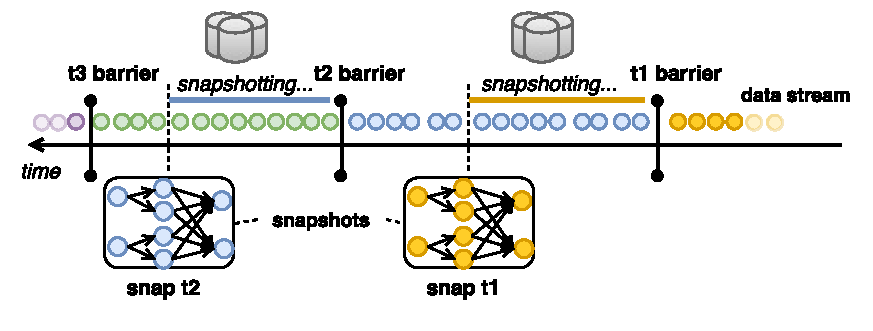
\includegraphics[width=.75\textwidth]{submissions/Bolong2023/figs/snaps.pdf}
% 	\caption{Test.}
% 	\label{bolong_fig:snapshots}
% \end{figure}

\subsection{Hybrid Queries}
Efficient ANN search algorithms have profoundly shaped a multitude of applications. However, as data becomes increasingly complex and multifaceted, there arose a need to refine these searches further, leading to the evolution of hybrid queries. 
For instance, consider an e-commerce platform where users search for products using both textual queries and specific attributes like price range, brand, or manufacturing date. While the primary search is still for products similar to a given product using textual similarity as the distance metric, hybrid quires require refining results further by considering the filters applied, ensuring that the results not only match the textual query but also fall within the specified price range, belong to the chosen brand, or were manufactured within the given date range. This introduces an additional layer of complexity into traditional ANN search.  


To address such hybrid queries, two straightforward ways are post-processing and pre-processing. The post-processing approach involves building a standard ANN search index, querying as usual, and then post-processing the results to select only those that align with the query filter. While simple, its performance is often found lacking in practical scenarios. Conversely, the pre-processing method involves building a distinct index for each possible filterable label, which can become infeasible with a large number of attribute constraints. 
Another intriguing method is inline-processing which integrates filter metadata with each vector into the index, and thus it simultaneously applies the filtering criteria as the search progresses through the dataset. Inline-processing can potentially offer more efficient results retrieval, but the state-of-the-art algorithms \cite{DBLP:journals/pvldb/WeiWWLZ0C20, DBLP:conf/osdi/ZhangXCSXCCH00Y23, DBLP:conf/www/GollapudiKSKBRL23} have yet to reach satisfactory levels. 


Optimizing algorithms for faster search, ensuring scalability for massive datasets, developing dynamic filtering mechanisms that can adapt to changing data landscapes, providing instant results for real-time applications like web search, and exploring the integration of deep learning techniques for enhanced accuracy are areas that need further improvement. Additionally, while the foundational concept remains intact, hybrid queries manifest in various forms, each customized to address specific application requirements. Some variants involve ANN searches with intricate predicates, while others demand the intersection of multiple ANN search results from distinct vector attributes. Some variants prioritize speed, while others might emphasize accuracy or the ability to handle dynamic datasets where data points can be added or removed frequently. All of these aspects remain open questions, beckoning further exploration and refinement.


\subsection{Out-of-Distribution Queries}
Out-of-distribution (OOD) queries refer to queries that are not drawn from the same distribution as the indexed data. 
A practical example of OOD is when a user searches through an image index using only a textual description as input. Even if both the image and text embeddings share the same representation space, the embeddings generated might lie in different distributions, leading to challenges in retrieval. State-of-the-art ANN search algorithms, such as graph-based and clustering-based indexes, achieve better query accuracy and efficiency over prior data-agnostic methods like LSH by employing data-dependent index construction. However, when the query data is OOD, there would be a significant performance decline due to the overfitting to the index data distribution.  By utilizing a small sample set drawn from the query distribution apriori, \cite{DBLP:journals/corr/abs-2211-12850} improves the mean query latency for OOD queries, but there is still much to explore and develop in this area. Handling OOD queries effectively is crucial for ensuring the robustness and reliability of AI systems, especially in critical applications. 
An ideal system should be able to generalize to OOD examples and flag those that are beyond its capability. It is  worth noting that OOD detection and handling are active areas of research, not only within the scope of ANN search, but also across various domains, spanning from computer vision to natural language processing.

\subsection{Data Series Similarity Search}
A data series is an ordered sequence of real numbers with length $l$. The most common type of data series is time series, where values are ordered by timestamp. This kind of data is exploding as the world is increasingly measured by sensors and other devices. Similarity search is a way to handle data series analysis task, such as anomaly detection, clustering and frequent pattern matching.

Data series can be treated as a special kind of high-dimensional vectors with ordered dimensions and high correlation between neighboring values. Similarly, exact and approximate $k$-nearest neighbors search problem can be defined for data series. However, except similarity metrics commonly used for high-dimensional vectors (Sec. \ref{bolong_sec:preliminaries}), there exist a few distance functions specialized for data series. For example, Dynamic Time Warping (DTW) \cite{DBLP:conf/kdd/RakthanmanonCMBWZZK12} automatically finds the correspondence between dimensions of two data series, which maximizes their similarity. Shape-based distance (SBD) \cite{DBLP:conf/sigmod/PaparrizosG15} slides one data series over the other and uses the maximum cross-correlation to determine their similarity. These methods may outperform Euclidean distance at some scenarios since they offer better alignment, yet also incur more computation overhead. Nevertheless, Euclidean distance still remains one of the most popular similarity metrics.

Over the years, the data series community has proposed many methods for data series similarity search, which are seldom considered and studied together with those for high-dimensional vectors until recently \cite{azizi2023elpis,DBLP:journals/pvldb/EchihabiFZPB22,DBLP:journals/pvldb/ChatzakisFKPP23}. Experiments conducted in \cite{DBLP:journals/pvldb/EchihabiZPB18,DBLP:journals/pvldb/EchihabiZPB19} compare the approaches from both communities and indicate that methods specialized for data series can achieve better performance. In addition, extensions are proposed to enable the existing data series indexes to support $\delta$-$\epsilon$-approximate search. 
It remains an open question if there exists a unified framework that can bridge the two worlds. 
%\textcolor{blue}{SOTA data series search methods are not included in the prominent vector database.}

\subsection{Scalability}
As we continue to generate and collect massive amounts of data in various domains, the scalability of vector databases becomes a critical concern \cite{DBLP:journals/tbd/JohnsonDJ21,DBLP:journals/jcisd/TingleTCGKDMI23,DBLP:journals/pvldb/ChatzakisFKPP23}. 
Consider the case of a global e-commerce platform, such as Taobao. Every day, Taobao collects vast amounts of data on user behavior, product details, transactions, and much more.
%The challenge of scalability is twofold: accommodating the explosively growing volume of high-dimensional data, and maintaining efficient, rapid query responses.
%
%\textbf{Handling High Volumes of Data}
%The digital universe is expanding at an unprecedented rate. As more industries and sectors embrace the use of machine learning and AI technologies, high-dimensional vector data is being produced and collected at a scale never seen before. In this context, vector databases must be designed to not only store but manage and manipulate these large volumes of data efficiently.
The traditional approach to handling large data volumes is to distribute the data across multiple nodes or servers \cite{DBLP:conf/cidr/CherniackBBCCXZ03}. However, distributing high-dimensional vector data is not straightforward. Unlike traditional relational data, where each record is independent and can be easily partitioned, high-dimensional vectors often need to be compared with one another during the similarity searches \cite{DBLP:journals/access/YangZCY19}, which complicates the distribution process. 
%
%
%\textbf{Maintaining Efficient Query Responses}
%Scalability is not just about storing more data; it's equally about delivering efficient query responses on this large-scale data. As the volume of data increases, ensuring that queries are processed and results are returned in a timely manner becomes increasingly challenging. 
Moreover, ANN search algorithms are commonly used in vector databases to speed up the search process. 
Existing algorithms use in-memory indexes for low latency and high throughput. However, as the data scales, these algorithms may still suffer from increased latency since it becomes expensive to load all the date into the memory and disk-based indexes must be considered. 
Furthermore, the infrastructure supporting the vector database will play a significant role in query performance. Techniques such as data sharding, load balancing, and efficient use of hardware will be crucial in ensuring that the system can handle high-concurrency, low-latency queries. 
DiskANN algorithms \cite{NEURIPS2019_09853c7f, DBLP:journals/corr/abs-2211-12850} index 5-10 times more points/machine using inexpensive SSDs with less than 10ms latency, which is close to the query latency in the in-memory indexes.
As we move into a future characterized by increasingly large volumes of high-dimensional data, research and development in this area will be crucial. Both data distribution strategies and query optimization techniques will need to evolve in tandem with the growing demands placed on these systems.


\subsection{Data Privacy and Security}
In the era of big data and machine learning, the issue of data privacy and security has taken center stage \cite{DBLP:conf/trustcom/GheidC16,DBLP:conf/ccs/WangLWTZ09}. 
%
%This is no less true for vector databases, where the high-dimensional data stored can often represent sensitive information. Ensuring the privacy and security of this data is a paramount concern, involving not just protection from unauthorized access, but also careful consideration of the privacy implications intrinsic to vector representations.
%
%\textbf{Protecting Vector Databases from Unauthorized Access.}
Like any database system, a vector database is potentially vulnerable to unauthorized access and data breaches. As vector databases become more widely used and the data they store becomes increasingly valuable, they will inevitably become attractive targets for cyber-attacks \cite{8355379}. This necessitates robust security measures to prevent unauthorized access.
Security protocols should include strong access controls, secure data transmission, and encryption strategies to protect the stored data. Moreover, constant monitoring and audit trails can help detect any suspicious activities. Implementing these measures requires a deep understanding of both database security and the specific vulnerabilities that may be unique to vector databases.
%
%\textbf{Privacy Implications of Vector Representations.}
Beyond the conventional concerns of data security, vector databases present another dimension of privacy challenge: the potential sensitivity of the vector representations themselves. High-dimensional vectors in these databases often capture meaningful patterns and structures in the data they represent. For instance, a vector could represent a user's behavior patterns, a patient's medical record, or a document's semantic content. This raises significant privacy concerns, as individuals might be identifiable from their corresponding vectors, even when the original data is anonymized.
A related concern is the potential for 'information leakage' from the vector representations . In some scenarios, it might be possible to reverse-engineer sensitive information from the vectors, especially if the method used to generate the vectors is known \cite{DBLP:journals/corr/abs-2205-10364}. This requires careful consideration of how vectors are generated and how they can be sufficiently anonymized or perturbed to prevent such leakage.
%These challenges will necessitate the development of new privacy-preserving techniques tailored to the context of vector databases. This might include methods for differential privacy, a mathematical technique that ensures the outputs of database queries do not reveal sensitive information about any individual record, or cryptographic techniques like homomorphic encryption that allows computations on encrypted data.
%%In conclusion, as the use of vector databases expands, the challenges of data privacy and security become more pressing. Future research and development in this area need to address both the traditional aspects of data security and the unique privacy concerns raised by high-dimensional vector representations. This will be critical in ensuring that vector databases can be used responsibly and ethically in a wide range of applications.

\subsection{Hardware Efficiency}
The growing dependence on vector databases for high-dimensional data processing has highlighted the importance of hardware efficiency. These databases often utilize approximate nearest neighbor (ANN) search algorithms to find similar vectors, resulting in a significant computational load. This challenge is further amplified in distributed systems that rely on GPUs, DRAM, and other hardware components, where fully utilizing hardware capabilities is crucial for performance but often difficult to achieve.
Recently, GPU-based ANN indexes such as SONG \cite{DBLP:conf/icde/ZhaoTL20} and GGNN \cite{DBLP:journals/tbd/GrohRWL23} have been proposed, achieving a two orders of magnitude speedup compared to CPU-based methods for ANN search. However, there are two factors to consider when delegating distance computation to GPUs. First, GPUs require interaction with the host's software and/or hardware layers, resulting in data transfer overhead for computation. Second, distance computations can be performed using a few simple, lightweight vector processing units, making GPUs a less cost-efficient choice for these tasks.
In addition, a software-hardware collaborative approach can combine software and hardware components to achieve highly scalable approximate nearest neighbor search services. A study called CXL-ANNS \cite{DBLP:conf/usenix/JangCBLKJ23} disaggregates DRAM from the host via Compute Express Link (CXL) and places all essential datasets into its memory pool. Another study, FANNS \cite{DBLP:journals/corr/abs-2306-11182}, automatically co-designs hardware and algorithms on FPGAs when given a user-provided recall requirement on a dataset and a hardware resource budget. Compared to purely CPU- or GPU-based methods, these software-hardware collaborative approaches achieve superior performance.



% \section{New Challenges and Opportunities}
% \label{bolong_sec:VectorDB}

% In this section, we will introduce high-dimensional data from LLM. We will discuss the scale and unique characteristics of high-dimensional data from LLM. Then we will discuss existing systems and research work, and identify research gaps. We will conclude with some concrete research plans.


\section{Conclusions}
\label{bolong_sec:conclusions}

As LLMs continue to be deployed in various domains, the demand for ANN search on vector representations is expected to surge exponentially. The current vector search libraries and database products still fall short of offering the comprehensive services on vector data. This underscores a significant gap and emphasizes the vast scope of work that remains to be addressed. In the near future, two main challenges may stand out: managing the scalability in the context of an exponentially increasing volume of vectors, and harnessing the potential of embedding models to enhance indexing and querying process. These challenges will likely be key areas of research moving forward. 


\section{Acknowledgments}
\label{bolong_sec:acknowledgements}

This work was partially conducted in the JC STEM Lab of Data Science Foundations funded by The Hong Kong Jockey Club Charities Trust, and was supported in part by NSFC (Grant No. 62372194), National Key Research and
Development Program of China under Grant No. 2021YFC3300303, Hubei Natural Science Foundation (Grant No. 2020CFB871), and Zilliz.
% Your bibliography must be included in your paper's single .tex file
% Do not included it via \include or via \bibtex 
% You can generate it using \bibtex, but put it into the paper here
% The bibliography must be less than two pages long.

% Do not change the commands below for your bibliography
% Keep font size and separator spacing
\bibliographystyle{plainnat}
\begin{thebibliography}{10}
\itemsep=1pt
\begin{small}

% Examples
% \bibitem{abadi2005design}
% D.~J. Abadi, Y.~Ahmad, M.~Balazinska, U.~Cetintemel, M.~Cherniack, J.-H. Hwang,
%   W.~Lindner, A.~Maskey, A.~Rasin, E.~Ryvkina, et~al.
% \newblock The design of the Borealis stream processing engine.
% \newblock {\em CIDR}, 2005.

% \bibitem{akidau2013millwheel}
% T.~Akidau, A.~Balikov, K.~Bekiro{\u{g}}lu, S.~Chernyak, J.~Haberman, R.~Lax,
%   S.~McVeety, D.~Mills, P.~Nordstrom, and S.~Whittle.
% \newblock Millwheel: fault-tolerant stream processing at Internet scale.
% \newblock {\em PVLDB}, 2013.

% \bibitem{akidau2015dataflow}
% T.~Akidau, R.~Bradshaw, C.~Chambers, S.~Chernyak, R.~J.
%   Fern{\'a}ndez-Moctezuma, R.~Lax, S.~McVeety, D.~Mills, F.~Perry, E.~Schmidt,
%   et~al.
% \newblock The dataflow model: a practical approach to balancing correctness,
%   latency, and cost in massive-scale, unbounded, out-of-order data processing.
% \newblock {\em PVLDB}, 2015.

\bibitem{DBLP:conf/stoc/IndykM98}
P. Indyk and R. Motwani.
\newblock Approximate Nearest Neighbors: Towards Removing the Curse of Dimensionality.
\newblock {\em STOC}, 1998.

\bibitem{DBLP:conf/vldb/GionisIM99}
A. Gionis, P. Indyk, and R. Motwani.
\newblock Similarity Search in High Dimensions via Hashing.
\newblock {\em VLDB}, 1999.

\bibitem{e2LSH}
A. Andoni and P. Indyk.
\newblock LSH algorithm and implementation (E2LSH).
\newblock { \url{https://www.mit.edu/~andoni/LSH}}, 2016.


\bibitem{DBLP:conf/compgeom/DatarIIM04}
M. Datar, N. Immorlica, P. Indyk, and V. S. Mirrokni.
\newblock Locality-sensitive hashing scheme based on p-stable distributions.
\newblock {\em Symposium on Computational Geometry}, 2004.

\bibitem{DBLP:conf/sigmod/TaoYSK09}
Y. Tao, K. Yi, C. Sheng, and P. Kalnis.
\newblock Quality and efficiency in high dimensional nearest neighbor search.
\newblock {\em SIGMOD}, 2009.

\bibitem{Multi-probe}
Q. Lv, W. Josephson, Z. Wang, M. Charikar, and K. Li.
\newblock Multi-probe LSH: efficient indexing for high-dimensional similarity search.
\newblock {\em VLDB}, 2007.

\bibitem{DBLP:conf/sigmod/LeiHKT20}
Y. Lei, Q. Huang, M. S. Kankanhalli, and A. K. H. Tung.
\newblock Locality-Sensitive Hashing Scheme based on Longest Circular Co-Substring.
\newblock {\em SIGMOD}, 2020.


\bibitem{DBLP:conf/sigmod/GanFFN12}
J. Gan, J. Feng, Q. Fang, and W. Ng.
\newblock Locality-sensitive hashing scheme based on dynamic collision counting.
\newblock {\em SIGMOD}, 2012.


\bibitem{DBLP:journals/pvldb/HuangFZFN15}
Q. Huang, J. Feng, Y. Zhang, Q. Fang, and W. Ng.
\newblock Query-Aware Locality-Sensitive Hashing for Approximate Nearest Neighbor.
\newblock {\em PVLDB}, 2015.

\bibitem{DBLP:conf/icde/LuK20}
K. Lu and M. Kudo.
\newblock R2LSH: A Nearest Neighbor Search Scheme Based on Two-dimensional.
\newblock {\em ICDE}, 2020.

\bibitem{DBLP:journals/pvldb/LuWWK20}
K. Lu, H. Wang, W. Wang, and M. Kudo.
\newblock VHP: Approximate Nearest Neighbor Search via Virtual Hypersphere.
\newblock {\em VLDB}, 2020.


\bibitem{DBLP:conf/icde/LiuWZWQ19}
W. Liu, H. Wang, Y. Zhang, W. Wang, and L. Qin.
\newblock I-LSH: I/O Efficient c-Approximate Nearest Neighbor Search in High-Dimensional Space.
\newblock {\em ICDE}, 2019.


\bibitem{DBLP:journals/vldb/LiuW00Q021}
W. Liu, H. Wang, Y. Zhang, W. Wang, L. Qin, and X. Lin.
\newblock EI-LSH: An early-termination driven {I/O} efficient incremental c-approximate nearest neighbor search.
\newblock {\em VLDB}, 2021.

\bibitem{DBLP:journals/pvldb/SunWQZL14}
Y. Sun, W. Wang, J. Qin, Y. Zhang, and X. Lin.
\newblock SRS: Solving c-Approximate Nearest Neighbor Queries in High Dimensional Euclidean Space with a Tiny Index.
\newblock {\em PVLDB}, 2014.



\bibitem{DBLP:journals/pvldb/ZhengZWHLJ20}
B. Zheng, X. Zhao, L. Weng, N. Q. V. Hung, H. Liu, and C. S. Jensen.
\newblock PM-LSH: A Fast and Accurate LSH Framework for High-Dimensional Approximate NN Search.
\newblock {\em Proc. VLDB Endow}, 2020.

\bibitem{DBLP:conf/focs/AndoniI06}
A. Andoni and P. Indyk.
\newblock Near-Optimal Hashing Algorithms for Approximate Nearest Neighbor in High Dimensions.
\newblock {\em FOCS}, 2006.

\bibitem{DBLP:conf/stoc/AndoniR15}
A. Andoni and I. P. Razenshtey.
\newblock Optimal Data-Dependent Hashing for Approximate Near Neighbors.
\newblock {\em STOC}, 2015.

\bibitem{DBLP:journals/tkde/LiWZWFLW23}
M. Li, Y. Wang, P. Zhang, H. Wang, L. Fan, E. Li, and W. Wang.
\newblock Deep Learning for Approximate Nearest Neighbour Search: A Survey and Future Directions.
\newblock {\em TKDE}, 2023.

\bibitem{DBLP:conf/icde/TianZZ22}
Y. Tian, X. Zhao, and X. Zhou.
\newblock DB-LSH: Locality-Sensitive Hashing with Query-based Dynamic Bucketing.
\newblock {\em ICDE}, 2022.

\bibitem{DB-LSH2}
Y. Tian, X. Zhao, and X. Zhou.
\newblock DB-LSH 2.0: Locality-Sensitive Hashing with Query-based Dynamic Bucketing.
\newblock {\em TKDE}, 2023.

\bibitem{DBLP:conf/www/BawaCG05}
Mayank Bawa, Tyson Condie, and Prasanna Ganesan.
\newblock LSH forest: self-tuning indexes for similarity search.
\newblock {\em WWW}, 2005.


\bibitem{DBLP:journals/pvldb/ZhaoZYLXZJ23}
X. Zhao, B. Zheng, X. Yi, X. Luan, C. Xie, X. Zhou, and C. S. Jensen.
\newblock FARGO: Fast Maximum Inner Product Search via Global Multi-Probing.
\newblock {\em PVLDB}, 2023.


\bibitem{DBLP:conf/sigmod/HuangLT21}
Q. Huang, Y. Lei, and A. K. H. Tung.
\newblock Point-to-Hyperplane Nearest Neighbor Search Beyond the Unit Hypersphere.
\newblock {\em SIGMOD}, 2021.



\bibitem{benchmark}
\newblock ANN Benchmarks.
\newblock { \url{https://ann-benchmarks.com/}}.


\bibitem{DBLP:journals/corr/abs-2211-12850}
S. Jaiswal, R. Krishnaswamy, A. Garg, H. V. Simhadri, and S. Agrawal.
\newblock OOD-DiskANN: Efficient and Scalable Graph {ANNS} for Out-of-Distribution Queries.
\newblock {\em CoRR}, 2022.

\bibitem{DBLP:conf/www/GollapudiKSKBRL23}
S. Gollapudi, N. Kari, V. Sivashankar, R. Krishnaswamy, N. Begwani, S. Raz, Y. Lin, Y. Zhang, N. Mahapatro, P. Srinivasan, A. Singh, and H. V. Simhadri.
\newblock Filtered-DiskANN: Graph Algorithms for Approximate Nearest Neighbor Search with Filters.
\newblock {\em WWW}, 2023.


\bibitem{DBLP:journals/pvldb/WeiWWLZ0C20}
C. Wei, B. Wu, S. Wang, R. Lou, C. Zhan, F. Li, and Y. Cai.
\newblock AnalyticDB-V: A Hybrid Analytical Engine Towards Query Fusion for Structured and Unstructured Data.
\newblock {\em PVLDB}, 2020.


\bibitem{DBLP:conf/osdi/ZhangXCSXCCH00Y23}
Q. Zhang, S. Xu, Q. Chen, G. Sui, J. Xie, Z. Cai, Y. Chen, Y. He, Y. Yang, F. Yang, M. Yang, and  L. Zhou.
\newblock VBASE: Unifying Online Vector Similarity Search and Relational Queries via Relaxed Monotonicity.
\newblock {\em OSDI}, 2023.








%%%%%PQ&Series%%%%%
\bibitem{DBLP:journals/pami/BabenkoL15}
A.~Babenko and V.~S. Lempitsky.
\newblock The inverted multi-index.
\newblock {\em {IEEE} Trans. Pattern Anal. Mach. Intell.}, 37(6):1247--1260,
2015.

\bibitem{DBLP:conf/cvpr/YandexL16}
A.~Babenko and V.~S. Lempitsky.
\newblock Efficient indexing of billion-scale datasets of deep descriptors.
\newblock In {\em {CVPR}}, pages 2055--2063. {IEEE} Computer Society, 2016.

\bibitem{DBLP:journals/pvldb/EchihabiZPB18}
K.~Echihabi, K.~Zoumpatianos, T.~Palpanas, and H.~Benbrahim.
\newblock The lernaean hydra of data series similarity search: An experimental
evaluation of the state of the art.
\newblock {\em Proc. {VLDB} Endow.}, 12(2):112--127, 2018.

\bibitem{DBLP:journals/pvldb/EchihabiZPB19}
K.~Echihabi, K.~Zoumpatianos, T.~Palpanas, and H.~Benbrahim.
\newblock Return of the lernaean hydra: Experimental evaluation of data series
approximate similarity search.
\newblock {\em Proc. {VLDB} Endow.}, 13(3):403--420, 2019.

\bibitem{DBLP:conf/cvpr/GeHK013}
T.~Ge, K.~He, Q.~Ke, and J.~Sun.
\newblock Optimized product quantization for approximate nearest neighbor
search.
\newblock In {\em {CVPR}}, pages 2946--2953. {IEEE} Computer Society, 2013.

\bibitem{8404126}
J.-P. Heo, Z.~Lin, and S.-E. Yoon.
\newblock Distance encoded product quantization for approximate k-nearest
neighbor search in high-dimensional space.
\newblock {\em IEEE Transactions on Pattern Analysis and Machine Intelligence},
41(9):2084--2097, 2019.

\bibitem{DBLP:journals/pami/JegouDS11}
H.~J{\'{e}}gou, M.~Douze, and C.~Schmid.
\newblock Product quantization for nearest neighbor search.
\newblock {\em {IEEE} Trans. Pattern Anal. Mach. Intell.}, 33(1):117--128,
2011.

\bibitem{DBLP:conf/cvpr/KalantidisA14}
Y.~Kalantidis and Y.~Avrithis.
\newblock Locally optimized product quantization for approximate nearest
neighbor search.
\newblock In {\em {CVPR}}, pages 2329--2336. {IEEE} Computer Society, 2014.

\bibitem{DBLP:conf/sigmod/LiZAH20}
C.~Li, M.~Zhang, D.~G. Andersen, and Y.~He.
\newblock Improving approximate nearest neighbor search through learned
adaptive early termination.
\newblock In {\em {SIGMOD} Conference}, pages 2539--2554. {ACM}, 2020.

\bibitem{Noh_2021_ICCV}
H.~Noh, T.~Kim, and J.-P. Heo.
\newblock Product quantizer aware inverted index for scalable nearest neighbor
search.
\newblock In {\em Proceedings of the IEEE/CVF International Conference on
	Computer Vision (ICCV)}, pages 12210--12218, October 2021.

\bibitem{DBLP:conf/sigmod/PaparrizosG15}
J.~Paparrizos and L.~Gravano.
\newblock k-shape: Efficient and accurate clustering of time series.
\newblock In {\em {SIGMOD} Conference}, pages 1855--1870. {ACM}, 2015.

\bibitem{DBLP:conf/kdd/RakthanmanonCMBWZZK12}
T.~Rakthanmanon, B.~J.~L. Campana, A.~Mueen, G.~E. A. P.~A. Batista, M.~B.
Westover, Q.~Zhu, J.~Zakaria, and E.~J. Keogh.
\newblock Searching and mining trillions of time series subsequences under
dynamic time warping.
\newblock In {\em {KDD}}, pages 262--270. {ACM}, 2012.

\bibitem{DBLP:conf/icde/ZhengYHYLX0J23}
B.~Zheng, Z.~Yue, Q.~Hu, X.~Yi, X.~Luan, C.~Xie, X.~Zhou, and C.~S. Jensen.
\newblock Learned probing cardinality estimation for high-dimensional
approximate {NN} search.
\newblock In {\em {ICDE}}, pages 3209--3221. {IEEE}, 2023.


%%%%% Xi %%%%%%%%%%%%%%%%%
\bibitem{faiss}
Faiss.
\newblock \url{https://github.com/facebookresearch/faiss}

\bibitem{nmslib}
NMSLib.
\newblock \url{https://github.com/nmslib/nmslib}

\bibitem{DBLP:conf/wims/BraticHKOR18}
B.~Bratic, M.~E. Houle, V.~Kurbalija, V.~Oria, and M.~Radovanovic.
\newblock Nn-descent on high-dimensional data.
\newblock In {\em {WIMS}}, pages 20:1--20:8, 2018.

\bibitem{DBLP:journals/corr/abs-2205-10364}
S.~Chen, H.~Khanpour, C.~Liu, and W.~Yang.
\newblock Learning to reverse dnns from {AI} programs automatically.
\newblock {\em CoRR}, abs/2205.10364, 2022.

\bibitem{DBLP:conf/cidr/CherniackBBCCXZ03}
M.~Cherniack, H.~Balakrishnan, M.~Balazinska, D.~Carney, U.~{\c{C}}etintemel,
Y.~Xing, and S.~B. Zdonik.
\newblock Scalable distributed stream processing.
\newblock In {\em {CIDR}}, 2003.

\bibitem{DBLP:journals/corr/FuC16}
C.~Fu and D.~Cai.
\newblock {EFANNA} : An extremely fast approximate nearest neighbor search
algorithm based on knn graph.
\newblock {\em CoRR}, abs/1609.07228, 2016.

\bibitem{DBLP:journals/pvldb/FuXWC19}
C.~Fu, C.~Xiang, C.~Wang, and D.~Cai.
\newblock Fast approximate nearest neighbor search with the navigating
spreading-out graph.
\newblock {\em {PVLDB}}, 12(5):461--474, 2019.

\bibitem{DBLP:conf/trustcom/GheidC16}
Z.~Gheid and Y.~Challal.
\newblock Efficient and privacy-preserving k-means clustering for big data
mining.
\newblock In {\em Trustcom/BigDataSE/ISPA}, pages 791--798. {IEEE}, 2016.

\bibitem{DBLP:journals/tbd/GrohRWL23}
F.~Groh, L.~Ruppert, P.~Wieschollek, and H.~P.~A. Lensch.
\newblock {GGNN:} graph-based {GPU} nearest neighbor search.
\newblock {\em {IEEE} Trans. Big Data}, 9(1):267--279, 2023.

\bibitem{8355379}
E.~Irmak and I.~Erkek.
\newblock An overview of cyber-attack vectors on scada systems.
\newblock In {\em 2018 6th International Symposium on Digital Forensic and
	Security (ISDFS)}, pages 1--5, 2018.

\bibitem{DBLP:conf/usenix/JangCBLKJ23}
J.~Jang, H.~Choi, H.~Bae, S.~Lee, M.~Kwon, and M.~Jung.
\newblock {CXL-ANNS:} software-hardware collaborative memory disaggregation and
computation for billion-scale approximate nearest neighbor search.
\newblock In {\em {USENIX} Annual Technical Conference}, pages 585--600.
{USENIX} Association, 2023.

\bibitem{DBLP:journals/dam/JaromczykK91}
J.~W. Jaromczyk and M.~Kowaluk.
\newblock Constructing the relative neighborhood graph in 3-dimensional
euclidean space.
\newblock {\em Discret. Appl. Math.}, 31(2):181--191, 1991.

\bibitem{NEURIPS2019_09853c7f}
S.~Jayaram~Subramanya, F.~Devvrit, H.~V. Simhadri, R.~Krishnawamy, and
R.~Kadekodi.
\newblock Diskann: Fast accurate billion-point nearest neighbor search on a
single node.
\newblock In {\em Advances in Neural Information Processing Systems},
volume~32. Curran Associates, Inc., 2019.

\bibitem{DBLP:journals/corr/abs-2306-11182}
W.~Jiang, S.~Li, Y.~Zhu, J.~de~Fine~Licht, Z.~He, R.~Shi, C.~Renggli, S.~Zhang,
T.~Rekatsinas, T.~Hoefler, and G.~Alonso.
\newblock Co-design hardware and algorithm for vector search.
\newblock {\em CoRR}, abs/2306.11182, 2023.

\bibitem{DBLP:journals/tbd/JohnsonDJ21}
J.~Johnson, M.~Douze, and H.~J{\'{e}}gou.
\newblock Billion-scale similarity search with gpus.
\newblock {\em {IEEE} Trans. Big Data}, 7(3):535--547, 2021.

\bibitem{DBLP:journals/corr/abs-1908-00814}
P.~Lin and W.~Zhao.
\newblock On the merge of k-nn graph.
\newblock {\em CoRR}, abs/1908.00814, 2019.

\bibitem{DBLP:journals/pami/MalkovY20}
Y.~A. Malkov and D.~A. Yashunin.
\newblock Efficient and robust approximate nearest neighbor search using
hierarchical navigable small world graphs.
\newblock {\em {IEEE} Trans. Pattern Anal. Mach. Intell.}, 42(4):824--836,
2020.

\bibitem{DBLP:journals/pr/MunozGDT19}
J.~A.~V. Mu{\~{n}}oz, M.~A. Gon{\c{c}}alves, Z.~Dias, and R.~da~Silva~Torres.
\newblock Hierarchical clustering-based graphs for large scale approximate
nearest neighbor search.
\newblock {\em Pattern Recognit.}, 96, 2019.

\bibitem{DBLP:journals/corr/abs-2105-09613}
A.~Singh, S.~J. Subramanya, R.~Krishnaswamy, and H.~V. Simhadri.
\newblock Freshdiskann: {A} fast and accurate graph-based {ANN} index for
streaming similarity search.
\newblock {\em CoRR}, abs/2105.09613, 2021.

\bibitem{DBLP:journals/jcisd/TingleTCGKDMI23}
B.~I. Tingle, K.~G. Tang, M.~Castanon, J.~J. Gutierrez, M.~Khurelbaatar,
C.~Dandarchuluun, Y.~S. Moroz, and J.~J. Irwin.
\newblock Zinc-22--a free multi-billion-scale database of tangible compounds
for ligand discovery.
\newblock {\em J. Chem. Inf. Model.}, 63(4):1166--1176, 2023.

\bibitem{DBLP:journals/pvldb/WangXY021}
M.~Wang, X.~Xu, Q.~Yue, and Y.~Wang.
\newblock A comprehensive survey and experimental comparison of graph-based
approximate nearest neighbor search.
\newblock {\em {PVLDB}}, 14(11):1964--1978, 2021.

\bibitem{DBLP:conf/ccs/WangLWTZ09}
R.~Wang, Y.~F. Li, X.~Wang, H.~Tang, and X.~Zhou.
\newblock Learning your identity and disease from research papers: information
leaks in genome wide association study.
\newblock In {\em {CCS}}, pages 534--544. {ACM}, 2009.

\bibitem{DBLP:journals/access/YangZCY19}
M.~Yang, Y.~Zuo, M.~Chen, and X.~Yu.
\newblock Scalable distributed knn processing on clustered data streams.
\newblock {\em {IEEE} Access}, 7:103198--103208, 2019.

\bibitem{DBLP:journals/corr/abs-1804-03032}
W.~Zhao.
\newblock k-nn graph construction: a generic online approach.
\newblock {\em CoRR}, abs/1804.03032, 2018.

\bibitem{DBLP:conf/icde/ZhaoTL20}
W.~Zhao, S.~Tan, and P.~Li.
\newblock {SONG:} approximate nearest neighbor search on {GPU}.
\newblock In {\em {ICDE}}, pages 1033--1044. {IEEE}, 2020.

\bibitem{DBLP:journals/pvldb/ZhaoTHZZ23}
X.~Zhao, Y.~Tian, K.~Huang, B.~Zheng, and X.~Zhou.
\newblock Towards efficient index construction and approximate nearest neighbor
search in high-dimensional spaces.
\newblock {\em Proc. {VLDB} Endow.}, 16(8):1979--1991, 2023.

\bibitem{annoy}
Bernhardsson, E. 
\newblock Annoy: Approximate Nearest Neighbors in C++/Python.
\newblock https://pypi.org/project/annoy/, Python package version 1.13.0, 2018

\bibitem{10.1109/TPAMI.2018.2889473}
Malkov, Y. \& Yashunin, D. 
\newblock Efficient and Robust Approximate Nearest Neighbor Search Using Hierarchical Navigable Small World Graphs. 
\newblock {\em IEEE Trans. Pattern Anal. Mach. Intell.} 42, 824-836, 2020 

\bibitem{SRS}
Sun, Y., Wang, W., Qin, J., Zhang, Y. \& Lin, X. 
\newblock SRS: Solving c-Approximate Nearest Neighbor Queries in High Dimensional Euclidean Space with a Tiny Index. 
\newblock {\em Proc. VLDB Endow.}. \textbf{8}, 1-12, 2014

\bibitem{xuemin_survey}
Li, W., Zhang, Y., Sun, Y., Wang, W., Li, M., Zhang, W. \& Lin, X. 
\newblock Approximate Nearest Neighbor Search on High Dimensional Data — Experiments, Analyses, and Improvement. 
\newblock {\em IEEE Transactions On Knowledge And Data Engineering}. \textbf{32}, 1475-1488, 2020

\bibitem{DBLP:conf/nips/BrownMRSKDNSSAA20}Brown, T., Mann, B., Ryder, N., Subbiah, M., Kaplan, J., et al. Language Models are Few-Shot Learners. {\em NeurIPS}. (2020)

\bibitem{DBLP:journals/corr/abs-2303-08774}OpenAI GPT-4 Technical Report. {\em CoRR}. {abs/2303.08774} (2023)

\bibitem{DBLP:conf/iclr/PatelLRCRC23}Patel, A., Li, B., Rasooli, M., Constant, N., Raffel, C. \& Callison-Burch, C. Bidirectional Language Models Are Also Few-shot Learners. {\em ICLR}. (2023)

\bibitem{pinecone}
Pinecone.
\newblock \url{https://docs.pinecone.io}

\bibitem{milvus}
Milvus.
\newblock \url{https://milvus.io/}


\bibitem{weaviate}
Weaviate.
\newblock \url{https://weaviate.io/}

\bibitem{azizi2023elpis}
Azizi, I., Echihabi, K. \& Palpanas, T. ELPIS: Graph-Based Similarity Search for Scalable Data Science. {\em Proceedings Of The VLDB Endowment}. \textbf{16}, 1548-1559 (2023)

\bibitem{DBLP:journals/pvldb/EchihabiFZPB22}
Echihabi, K., Fatourou, P., Zoumpatianos, K., Palpanas, T. \& Benbrahim, H. Hercules Against Data Series Similarity Search. {\em Proc. VLDB Endow.}. \textbf{15}, 2005-2018 (2022)

\bibitem{DBLP:journals/pvldb/ChatzakisFKPP23}Chatzakis, M., Fatourou, P., Kosmas, E., Palpanas, T. \& Peng, B. Odyssey: A Journey in the Land of Distributed Data Series Similarity Search. {\em Proc. VLDB Endow.}. \textbf{16}, 1140-1153 (2023)
\end{small}
\end{thebibliography}


%\balance
%\bibliographystyle{abbrv}
%%\bibliographystyle{ACM-Reference-Format}
%\bibliography{references}
%\bibliography{myRef}
% {
% \small
% \bibliographystyle{abbrv}
% \bibliography{myRef_used}
% }
% \printbibliography

\end{document}